\documentclass[twoside]{book}

% Packages required by doxygen
\usepackage{fixltx2e}
\usepackage{calc}
\usepackage{doxygen}
\usepackage[export]{adjustbox} % also loads graphicx
\usepackage{graphicx}
\usepackage[utf8]{inputenc}
\usepackage{makeidx}
\usepackage{multicol}
\usepackage{multirow}
\PassOptionsToPackage{warn}{textcomp}
\usepackage{textcomp}
\usepackage[nointegrals]{wasysym}
\usepackage[table]{xcolor}

% Font selection
\usepackage[T1]{fontenc}
\usepackage[scaled=.90]{helvet}
\usepackage{courier}
\usepackage{amssymb}
\usepackage{sectsty}
\renewcommand{\familydefault}{\sfdefault}
\allsectionsfont{%
  \fontseries{bc}\selectfont%
  \color{darkgray}%
}
\renewcommand{\DoxyLabelFont}{%
  \fontseries{bc}\selectfont%
  \color{darkgray}%
}
\newcommand{\+}{\discretionary{\mbox{\scriptsize$\hookleftarrow$}}{}{}}

% Page & text layout
\usepackage{geometry}
\geometry{%
  a4paper,%
  top=2.5cm,%
  bottom=2.5cm,%
  left=2.5cm,%
  right=2.5cm%
}
\tolerance=750
\hfuzz=15pt
\hbadness=750
\setlength{\emergencystretch}{15pt}
\setlength{\parindent}{0cm}
\setlength{\parskip}{3ex plus 2ex minus 2ex}
\makeatletter
\renewcommand{\paragraph}{%
  \@startsection{paragraph}{4}{0ex}{-1.0ex}{1.0ex}{%
    \normalfont\normalsize\bfseries\SS@parafont%
  }%
}
\renewcommand{\subparagraph}{%
  \@startsection{subparagraph}{5}{0ex}{-1.0ex}{1.0ex}{%
    \normalfont\normalsize\bfseries\SS@subparafont%
  }%
}
\makeatother

% Headers & footers
\usepackage{fancyhdr}
\pagestyle{fancyplain}
\fancyhead[LE]{\fancyplain{}{\bfseries\thepage}}
\fancyhead[CE]{\fancyplain{}{}}
\fancyhead[RE]{\fancyplain{}{\bfseries\leftmark}}
\fancyhead[LO]{\fancyplain{}{\bfseries\rightmark}}
\fancyhead[CO]{\fancyplain{}{}}
\fancyhead[RO]{\fancyplain{}{\bfseries\thepage}}
\fancyfoot[LE]{\fancyplain{}{}}
\fancyfoot[CE]{\fancyplain{}{}}
\fancyfoot[RE]{\fancyplain{}{\bfseries\scriptsize Generated by Doxygen }}
\fancyfoot[LO]{\fancyplain{}{\bfseries\scriptsize Generated by Doxygen }}
\fancyfoot[CO]{\fancyplain{}{}}
\fancyfoot[RO]{\fancyplain{}{}}
\renewcommand{\footrulewidth}{0.4pt}
\renewcommand{\chaptermark}[1]{%
  \markboth{#1}{}%
}
\renewcommand{\sectionmark}[1]{%
  \markright{\thesection\ #1}%
}

% Indices & bibliography
\usepackage{natbib}
\usepackage[titles]{tocloft}
\setcounter{tocdepth}{3}
\setcounter{secnumdepth}{5}
\makeindex

% Hyperlinks (required, but should be loaded last)
\usepackage{ifpdf}
\ifpdf
  \usepackage[pdftex,pagebackref=true]{hyperref}
\else
  \usepackage[ps2pdf,pagebackref=true]{hyperref}
\fi
\hypersetup{%
  colorlinks=true,%
  linkcolor=blue,%
  citecolor=blue,%
  unicode%
}

% Custom commands
\newcommand{\clearemptydoublepage}{%
  \newpage{\pagestyle{empty}\cleardoublepage}%
}

\usepackage{caption}
\captionsetup{labelsep=space,justification=centering,font={bf},singlelinecheck=off,skip=4pt,position=top}

%===== C O N T E N T S =====

\begin{document}

% Titlepage & ToC
\hypersetup{pageanchor=false,
             bookmarksnumbered=true,
             pdfencoding=unicode
            }
\pagenumbering{alph}
\begin{titlepage}
\vspace*{7cm}
\begin{center}%
{\Large Tokenika eosc \\[1ex]\large 0.\+5 }\\
\vspace*{1cm}
{\large Generated by Doxygen 1.8.13}\\
\end{center}
\end{titlepage}
\clearemptydoublepage
\pagenumbering{roman}
\tableofcontents
\clearemptydoublepage
\pagenumbering{arabic}
\hypersetup{pageanchor=true}

%--- Begin generated contents ---
\chapter{Tokenika alternative for the E\+OS $\ast$eosc$\ast$ program}
\label{autotoc_md0}
\Hypertarget{autotoc_md0}
\label{_toc}%
 \subsection*{Table of contents}


\begin{DoxyItemize}
\item \href{#rationale}{\tt Rationale}
\begin{DoxyItemize}
\item \href{#richer}{\tt Richer A\+PI}
\begin{DoxyItemize}
\item \href{#richereos}{\tt E\+OS}
\item \href{#richertokenika}{\tt Tokenika}
\end{DoxyItemize}
\end{DoxyItemize}
\item \href{#building}{\tt Building}
\begin{DoxyItemize}
\item \href{#dependencies}{\tt Dependencies}
\item \href{#linux}{\tt Linux, Mac, ect.}
\item \href{#windows}{\tt Windows}
\end{DoxyItemize}
\end{DoxyItemize}

\label{_rationale}%
 \subsection*{\href{#toc}{\tt Rationale}}

For our work with eos small contracts, we have found that the original E\+OS {\ttfamily eosc} interface program is too much restrictive. First, it is hard to be used programmatically in a C++ code. Next, it is quite heavy as it is tightly connected to the whole of the E\+OS code. Also, it is not ready to be used in the Windows environment, while we plan to open Windows based contract development possibility.

It could be enough for us to develope a minimal C++ library, implementing the commands of the E\+OS {\ttfamily eosc}. However, it was a short step to to provide this library with an command line interface.

Finally, to make our work competitive to the original, and for fun, we have added a richer command option list. We dare to hope that this little work of ours could be included to the E\+OS project.

We already know how to use this richness\+: it is much ease to make a tool as tokenika \href{#}{\tt {\ttfamily eosc\+Bash}} that wraps the E\+OS {\ttfamily eosc} for bookkeeping.

\label{_richer}%
 \subsection*{\href{#toc}{\tt Richer A\+PI}}

\label{_richereos}%
 \#\#\# \href{#toc}{\tt E\+OS} 
\begin{DoxyCode}
./eosc get block -h
\end{DoxyCode}
 
\begin{DoxyCode}
ERROR: RequiredError: block
Retrieve a full block from the blockchain
Usage: ./eosc get block block

Positionals:
  block TEXT                  The number or ID of the block to retrieve
\end{DoxyCode}
 
\begin{DoxyCode}
./eosc get block 25
\end{DoxyCode}
 
\begin{DoxyCode}
\{
  "previous": "00000018b5e0ffcd3dfede45bc261e3a04de9f1f40386a69821780e063a41448",
  "timestamp": "2017-11-29T09:50:03",
  "transaction\_merkle\_root": "0000000000000000000000000000000000000000000000000000000000000000",
  "producer": "initf",
  "producer\_changes": [],
  "producer\_signature":
       "2005db1a193cc3597fdc3bd38a4375df2a9f9593390f9431f7a9b53701cd46a1b5418b9cd68edbdf2127d6ececc4d66b7a190e72a97ce9adfcc750ef0a770f5619",
  "cycles": [],
  "id": "000000190857c9fb43d62525bd29dc321003789c075de593ce7224bde7fc2284",
  "block\_num": 25,
  "refBlockPrefix": 623236675
\}
\end{DoxyCode}


\label{_richtokenika}%
 \subsubsection*{Tokenika}


\begin{DoxyCode}
./eosc get block -h
\end{DoxyCode}
 
\begin{DoxyCode}
Retrieve a full block from the blockchain
Usage: ./eosc get block [block\_num] [Options]
Usage: ./eosc get block [-j \{"block\_num\_or\_id":*\}] [OPTIONS]

Options:

  -n [ --block\_num ] arg  Block number
  -i [ --block\_id ] arg   Block id

  -h [ --help ]           Help screen
  -j [ --json ] arg       Json argument
  -v [ --received ]       Print received json
  -r [ --raw ]            Not pretty print
  -e [ --example ]        Usage example
\end{DoxyCode}
 
\begin{DoxyCode}
./eosc get block 25
##         block number: 25
##            timestamp: 2017-11-29T09:50:03
##     ref block prefix: 623236675
\end{DoxyCode}
 
\begin{DoxyCode}
./eosc get block 25 -v
\end{DoxyCode}
 
\begin{DoxyCode}
\{
    "previous": "00000018b5e0ffcd3dfede45bc261e3a04de9f1f40386a69821780e063a41448",
    "timestamp": "2017-11-29T09:50:03",
    "transaction\_merkle\_root": "0000000000000000000000000000000000000000000000000000000000000000",
    "producer": "initf",
    "producer\_changes": "",
    "producer\_signature":
       "2005db1a193cc3597fdc3bd38a4375df2a9f9593390f9431f7a9b53701cd46a1b5418b9cd68edbdf2127d6ececc4d66b7a190e72a97ce9adfcc750ef0a770f5619",
    "cycles": "",
    "id": "000000190857c9fb43d62525bd29dc321003789c075de593ce7224bde7fc2284",
    "block\_num": "25",
    "refBlockPrefix": "623236675"
\}
\end{DoxyCode}
 
\begin{DoxyCode}
./eosc get block 25 -v -r
\end{DoxyCode}
 
\begin{DoxyCode}

      \{"previous":"00000018b5e0ffcd3dfede45bc261e3a04de9f1f40386a69821780e063a41448","timestamp":"2017-11-29T09:50
      :03","transaction\_merkle\_root":"0000000000000000000000000000000000000000000000000000000000000000","producer"
      :"initf","producer\_changes":"","producer\_signature":"2005db1a193cc3597fdc3bd38a4375df2a9f9593390f9431f7a9b53
      701cd46a1b5418b9cd68edbdf2127d6ececc4d66b7a190e72a97ce9adfcc750ef0a770f5619","cycles":"","id":"000000190857c9fb43d62525bd29dc321003789c075de593ce7224bde7fc2284","block\_num":"25","refBlockPrefix":"623236675"\}
\end{DoxyCode}
 
\begin{DoxyCode}
./eosc get block -j '\{"block\_num\_or\_id":"56"\}'
##         block number: 56
##            timestamp: 2017-11-29T10:02:18
##     ref block prefix: 273573026
\end{DoxyCode}
 
\begin{DoxyCode}
./eosc get block --example
\end{DoxyCode}
 
\begin{DoxyCode}
Invoke 'get\_info' command:
get\_info get\_info;

\{
    "head\_block\_num": "9939",
    "last\_irreversible\_block\_num": "9924",
    "head\_block\_id": "000026d378f90b5d25dcf962fc44d637872218e5f826420a342f05a534d50bfc",
    "head\_block\_time": "2017-12-01T18:57:42",
    "head\_block\_producer": "initr",
    "recent\_slots": "0000000000000000000000000000000000000000000000000011111111111111",
    "participation\_rate": "0.21875000000000000"
\}


Use reference to the last block:
GetBlock GetBlock(
  get\_info.get<int>("last\_irreversible\_block\_num"));

\{
    "previous": "000026c35fb5d442be6d4e81a1347cce2c0184c4c2047d9e6dfc78b3bb325ac2",
    "timestamp": "2017-12-01T17:01:09",
    "transaction\_merkle\_root": "0000000000000000000000000000000000000000000000000000000000000000",
    "producer": "initn",
    "producer\_changes": "",
    "producer\_signature":
       "1f6984d14ee40ed9806ae14aa96531d874fc3417bf3f1b66c4b1d9c9402f3f90ef07c4523eb9a639ad632c181580aeb051385d718dc59ecc54d0f0e5de012b540f",
    "cycles": "",
    "id": "000026c44a2e8075a5b92813869bfb67b72b79ccb3f2e40ad815603c04d2fafd",
    "block\_num": "9924",
    "refBlockPrefix": "321436069"
\}
\end{DoxyCode}
 \subsection*{Library}

For us, real value is the library that runs the {\ttfamily tokenika eosc}, as we see the original eos library as not practical for our work. We need a light-\/weight thing, a cross-\/platform (good for windows) one.

Let you see a code snippet\+: 
\begin{DoxyCode}
#include <stdio.h>
#include <stdlib.h>
#include <iostream>
#include <string>

#include "EoscCommands/eosc\_get\_commands.hpp"

int main(int argc, char *argv[])
\{
  tokenika::eosc::get\_info get\_info; /* Call 'eosd' for 'get info'. */
  tokenika::eosc::GetBlock GetBlock( /* Call 'eosd' for 'get block', the last one. */
    get\_info.get<int>("last\_irreversible\_block\_num"));

  std::cout << GetBlock.toStringRcv() << std::endl;/* Print the response. */

  return 0;
\}
\end{DoxyCode}
 Here is the print-\/out\+: 
\begin{DoxyCode}
    "previous": "000028716589219b442afe9d140bc28eff4335aecd37d519b0105fca4c8e4a3f",
    "timestamp": "2017-12-01T19:18:27",
    "transaction\_merkle\_root": "0000000000000000000000000000000000000000000000000000000000000000",
    "producer": "inith",
    "producer\_changes": "",
    "producer\_signature":
       "1f510dec0bcd85847b7bead61f6deee7a5fb4108745e6ceaaa81804fe4700b561f7ca3f3f26f56fbfaf1e10fd3ba2999f8cbe165fd391b023334badcf894ba54dc",
    "cycles": "",
    "id": "00002872be99d0133ea104b42b771f3c7c2ea3736263dc9db3719728a2776976",
    "block\_num": "10354",
    "refBlockPrefix": "3020202302"
\}
\end{DoxyCode}


\label{_building}%
 \subsection*{\href{#toc}{\tt Building}}

\label{_dependencies}%
 \subsubsection*{\href{#toc}{\tt Dependencies}}

The only external dependency is the boost. We use the version 1\+\_\+65.

\label{_linux}%
 \subsubsection*{\href{#toc}{\tt Linux, Mac, ect.}}

C\+Make build. Starting in the installation directory\+:


\begin{DoxyCode}
mkdir build
cd build
cmake ..
make
\end{DoxyCode}


\label{_windows}%
 \subsubsection*{\href{#toc}{\tt Windows}}

There is an MS Visual Studio 17 solution in {\ttfamily eos\+\_\+visual\+\_\+studio} folder. You can start Visual Studio with file {\ttfamily eosc.\+sln} there, and you compile both the command library and `eosc\textquotesingle{} executable.

The VS solution has set both boost includes and libraries in relation to the {\ttfamily B\+O\+O\+S\+T\+\_\+\+R\+O\+OT} environmental variable\+: Configuration Properties $>$ V\+C++ Directories. Perhaps, you will have to adjust settings.

Now, the blockchain may be accessed from a Windows Command Prompt, if the {\ttfamily eosd} blockchain program is configured to be called from 
\chapter{Hierarchical Index}
\section{Class Hierarchy}
This inheritance list is sorted roughly, but not completely, alphabetically\+:\begin{DoxyCompactList}
\item \contentsline{section}{tokenika\+:\+:eosc\+:\+:Command\+Options}{\pageref{classtokenika_1_1eosc_1_1_command_options}}{}
\begin{DoxyCompactList}
\item \contentsline{section}{tokenika\+:\+:eosc\+:\+:Get\+Block\+Options}{\pageref{classtokenika_1_1eosc_1_1_get_block_options}}{}
\item \contentsline{section}{tokenika\+:\+:eosc\+:\+:Get\+Info\+Options}{\pageref{classtokenika_1_1eosc_1_1_get_info_options}}{}
\end{DoxyCompactList}
\item \contentsline{section}{tokenika\+:\+:eosc\+:\+:Eosc\+Command}{\pageref{classtokenika_1_1eosc_1_1_eosc_command}}{}
\begin{DoxyCompactList}
\item \contentsline{section}{tokenika\+:\+:eosc\+:\+:Get\+Block}{\pageref{classtokenika_1_1eosc_1_1_get_block}}{}
\item \contentsline{section}{tokenika\+:\+:eosc\+:\+:Get\+Info}{\pageref{classtokenika_1_1eosc_1_1_get_info}}{}
\end{DoxyCompactList}
\item \contentsline{section}{tokenika\+:\+:eosc\+:\+:Init\+Get\+Json}{\pageref{structtokenika_1_1eosc_1_1_init_get_json}}{}
\item \contentsline{section}{server}{\pageref{classserver}}{}
\item \contentsline{section}{session}{\pageref{classsession}}{}
\end{DoxyCompactList}

\chapter{Data Structure Index}
\section{Data Structures}
Here are the data structures with brief descriptions\+:\begin{DoxyCompactList}
\item\contentsline{section}{\hyperlink{classtokenika_1_1eosc_1_1_command_options}{tokenika\+::eosc\+::\+Command\+Options} \\*Command-\/line wrapper for eosc commands }{\pageref{classtokenika_1_1eosc_1_1_command_options}}{}
\item\contentsline{section}{\hyperlink{classtokenika_1_1eosc_1_1_eosc_command}{tokenika\+::eosc\+::\+Eosc\+Command} \\*Basic connection to the blockchain }{\pageref{classtokenika_1_1eosc_1_1_eosc_command}}{}
\item\contentsline{section}{\hyperlink{classtokenika_1_1eosc_1_1_get_block}{tokenika\+::eosc\+::\+Get\+Block} \\*Retrieve a full block from a blockchain }{\pageref{classtokenika_1_1eosc_1_1_get_block}}{}
\item\contentsline{section}{\hyperlink{classtokenika_1_1eosc_1_1_get_block_options}{tokenika\+::eosc\+::\+Get\+Block\+Options} }{\pageref{classtokenika_1_1eosc_1_1_get_block_options}}{}
\item\contentsline{section}{\hyperlink{classtokenika_1_1eosc_1_1_get_info}{tokenika\+::eosc\+::\+Get\+Info} \\*Get current blockchain information }{\pageref{classtokenika_1_1eosc_1_1_get_info}}{}
\item\contentsline{section}{\hyperlink{classtokenika_1_1eosc_1_1_get_info_options}{tokenika\+::eosc\+::\+Get\+Info\+Options} }{\pageref{classtokenika_1_1eosc_1_1_get_info_options}}{}
\item\contentsline{section}{\hyperlink{structtokenika_1_1eosc_1_1_init_get_json}{tokenika\+::eosc\+::\+Init\+Get\+Json} }{\pageref{structtokenika_1_1eosc_1_1_init_get_json}}{}
\item\contentsline{section}{\hyperlink{classserver}{server} }{\pageref{classserver}}{}
\item\contentsline{section}{\hyperlink{classsession}{session} }{\pageref{classsession}}{}
\end{DoxyCompactList}

\chapter{File Index}
\section{File List}
Here is a list of all documented files with brief descriptions\+:\begin{DoxyCompactList}
\item\contentsline{section}{{\bfseries boost\+\_\+tdd1/const\+\_\+string.\+hpp} }{\pageref{boost__tdd1_2const__string_8hpp}}{}
\item\contentsline{section}{{\bfseries boost\+\_\+tdd2/const\+\_\+string.\+hpp} }{\pageref{boost__tdd2_2const__string_8hpp}}{}
\item\contentsline{section}{{\bfseries eosc.\+hpp} }{\pageref{eosc_8hpp}}{}
\item\contentsline{section}{\hyperlink{eosc__command_8hpp}{eosc\+\_\+command.\+hpp} \\*Tool for sending transactions and querying state from E\+OS blockchain }{\pageref{eosc__command_8hpp}}{}
\item\contentsline{section}{{\bfseries eosc\+\_\+config.\+h} }{\pageref{eosc__config_8h}}{}
\item\contentsline{section}{\hyperlink{eosc__get__commands_8hpp}{eosc\+\_\+get\+\_\+commands.\+hpp} }{\pageref{eosc__get__commands_8hpp}}{}
\item\contentsline{section}{{\bfseries eosc\+\_\+test.\+hpp} }{\pageref{eosc__test_8hpp}}{}
\item\contentsline{section}{{\bfseries asyn\+\_\+tcp\+\_\+echo\+\_\+server/targetver.\+h} }{\pageref{asyn__tcp__echo__server_2targetver_8h}}{}
\item\contentsline{section}{{\bfseries blocking\+\_\+tcp\+\_\+echo\+\_\+client/targetver.\+h} }{\pageref{blocking__tcp__echo__client_2targetver_8h}}{}
\item\contentsline{section}{{\bfseries boost\+\_\+tdd1/targetver.\+h} }{\pageref{boost__tdd1_2targetver_8h}}{}
\item\contentsline{section}{{\bfseries boost\+\_\+tdd2/targetver.\+h} }{\pageref{boost__tdd2_2targetver_8h}}{}
\item\contentsline{section}{{\bfseries eosc/targetver.\+h} }{\pageref{eosc_2targetver_8h}}{}
\item\contentsline{section}{{\bfseries eosc\+Lib/targetver.\+h} }{\pageref{eosc_lib_2targetver_8h}}{}
\item\contentsline{section}{{\bfseries firewall\+\_\+tunnel/targetver.\+h} }{\pageref{firewall__tunnel_2targetver_8h}}{}
\item\contentsline{section}{{\bfseries test.\+hpp} }{\pageref{test_8hpp}}{}
\end{DoxyCompactList}

\chapter{Data Structure Documentation}
\hypertarget{classtokenika_1_1eosc_1_1_command_options}{}\section{tokenika\+:\+:eosc\+:\+:Command\+Options Class Reference}
\label{classtokenika_1_1eosc_1_1_command_options}\index{tokenika\+::eosc\+::\+Command\+Options@{tokenika\+::eosc\+::\+Command\+Options}}


Command-\/line wrapper for eosc commands.  




{\ttfamily \#include $<$eosc\+\_\+command.\+hpp$>$}



Inheritance diagram for tokenika\+:\+:eosc\+:\+:Command\+Options\+:\nopagebreak
\begin{figure}[H]
\begin{center}
\leavevmode
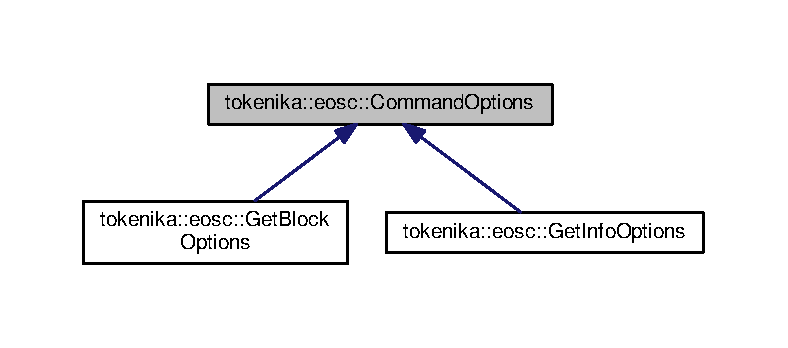
\includegraphics[width=350pt]{classtokenika_1_1eosc_1_1_command_options__inherit__graph}
\end{center}
\end{figure}
\subsection*{Public Member Functions}
\begin{DoxyCompactItemize}
\item 
\mbox{\Hypertarget{classtokenika_1_1eosc_1_1_command_options_a61d20e4e3a9564c242eecfe814e96783}\label{classtokenika_1_1eosc_1_1_command_options_a61d20e4e3a9564c242eecfe814e96783}} 
{\bfseries Command\+Options} (int argc, const char $\ast$argv\mbox{[}$\,$\mbox{]})
\item 
\mbox{\Hypertarget{classtokenika_1_1eosc_1_1_command_options_a4fa1c9defc45b139e415c79c43b15e5d}\label{classtokenika_1_1eosc_1_1_command_options_a4fa1c9defc45b139e415c79c43b15e5d}} 
void {\bfseries go} ()
\end{DoxyCompactItemize}
\subsection*{Protected Member Functions}
\begin{DoxyCompactItemize}
\item 
virtual const char $\ast$ \hyperlink{classtokenika_1_1eosc_1_1_command_options_a18ada0ba1163f7a41c9990ae2756012b}{get\+Usage} ()
\begin{DoxyCompactList}\small\item\em Command \textquotesingle{}usage\textquotesingle{} instruction. \end{DoxyCompactList}\item 
virtual boost\+::program\+\_\+options\+::options\+\_\+description \hyperlink{classtokenika_1_1eosc_1_1_command_options_aa55960f380250eb7065cb6489b67196f}{options} ()
\begin{DoxyCompactList}\small\item\em List of the command options. \end{DoxyCompactList}\item 
virtual void \hyperlink{classtokenika_1_1eosc_1_1_command_options_ae2e98c683ae1eb3e5af1e81e60020447}{set\+Pos\+Desc} (boost\+::program\+\_\+options\+::positional\+\_\+options\+\_\+description \&pos\+\_\+descr)
\begin{DoxyCompactList}\small\item\em Positional options. \end{DoxyCompactList}\item 
virtual bool \hyperlink{classtokenika_1_1eosc_1_1_command_options_a7aecc9aa79ca65f6abbd568ff8ff77a7}{set\+Json} (boost\+::program\+\_\+options\+::variables\+\_\+map \&vm)
\begin{DoxyCompactList}\small\item\em Fills the post json tree according to options. \end{DoxyCompactList}\item 
virtual \hyperlink{classtokenika_1_1eosc_1_1_eosc_command}{Eosc\+Command} \hyperlink{classtokenika_1_1eosc_1_1_command_options_a787f15164e2055394d9d948c07bf201c}{get\+Command} (bool is\+Raw)
\begin{DoxyCompactList}\small\item\em Returns command object, containing a responce frosource /mnt/hgfs/\+Workspaces/\+E\+O\+S/eosc\+Bash/eosc\+Bash \$\+E\+O\+S\+I\+O\+\_\+\+I\+N\+S\+T\+A\+L\+L\+\_\+\+D\+IR m the blockchain. \end{DoxyCompactList}\item 
virtual void \hyperlink{classtokenika_1_1eosc_1_1_command_options_ab1fe134b6c2230257a5c07b021812986}{get\+Example} ()
\begin{DoxyCompactList}\small\item\em Placeholder for any exemplary code snippet. \end{DoxyCompactList}\item 
virtual void \hyperlink{classtokenika_1_1eosc_1_1_command_options_a346dcfb00b8ac522169714544bfa7be0}{get\+Output} (\hyperlink{classtokenika_1_1eosc_1_1_eosc_command}{Eosc\+Command} command)
\begin{DoxyCompactList}\small\item\em Placeholder for printout instructions. \end{DoxyCompactList}\end{DoxyCompactItemize}
\subsection*{Protected Attributes}
\begin{DoxyCompactItemize}
\item 
\mbox{\Hypertarget{classtokenika_1_1eosc_1_1_command_options_a626e842c89d8332090886bc53fbad616}\label{classtokenika_1_1eosc_1_1_command_options_a626e842c89d8332090886bc53fbad616}} 
boost\+::property\+\_\+tree\+::ptree \hyperlink{classtokenika_1_1eosc_1_1_command_options_a626e842c89d8332090886bc53fbad616}{post\+Json}
\begin{DoxyCompactList}\small\item\em json tree to be filled with blockchain responce. \end{DoxyCompactList}\end{DoxyCompactItemize}


\subsection{Detailed Description}
Command-\/line wrapper for eosc commands. 

The prototype for command-\/line wrappers for eosc commands. Defines common options like \textquotesingle{}help\textquotesingle{}, \textquotesingle{}example\textquotesingle{}.

Also, the class defines virtual methods that are placeholders for specific definitions of the command that is wrapped. 

\subsection{Member Function Documentation}
\mbox{\Hypertarget{classtokenika_1_1eosc_1_1_command_options_a787f15164e2055394d9d948c07bf201c}\label{classtokenika_1_1eosc_1_1_command_options_a787f15164e2055394d9d948c07bf201c}} 
\index{tokenika\+::eosc\+::\+Command\+Options@{tokenika\+::eosc\+::\+Command\+Options}!get\+Command@{get\+Command}}
\index{get\+Command@{get\+Command}!tokenika\+::eosc\+::\+Command\+Options@{tokenika\+::eosc\+::\+Command\+Options}}
\subsubsection{\texorpdfstring{get\+Command()}{getCommand()}}
{\footnotesize\ttfamily virtual \hyperlink{classtokenika_1_1eosc_1_1_eosc_command}{Eosc\+Command} tokenika\+::eosc\+::\+Command\+Options\+::get\+Command (\begin{DoxyParamCaption}\item[{bool}]{is\+Raw }\end{DoxyParamCaption})\hspace{0.3cm}{\ttfamily [inline]}, {\ttfamily [protected]}, {\ttfamily [virtual]}}



Returns command object, containing a responce frosource /mnt/hgfs/\+Workspaces/\+E\+O\+S/eosc\+Bash/eosc\+Bash \$\+E\+O\+S\+I\+O\+\_\+\+I\+N\+S\+T\+A\+L\+L\+\_\+\+D\+IR m the blockchain. 


\begin{DoxyParams}{Parameters}
{\em is\+Raw} & raw or pretty printout flag \\
\hline
\end{DoxyParams}
\begin{DoxyReturn}{Returns}
\hyperlink{classtokenika_1_1eosc_1_1_eosc_command}{Eosc\+Command} command object 
\end{DoxyReturn}


Reimplemented in \hyperlink{classtokenika_1_1eosc_1_1_get_block_options_ac1c5b62f162c4253cab8de5a93fe5cf9}{tokenika\+::eosc\+::\+Get\+Block\+Options}, and \hyperlink{classtokenika_1_1eosc_1_1_get_info_options_a7283bdc9a328ccd8a29a25bcdc01dfa6}{tokenika\+::eosc\+::\+Get\+Info\+Options}.

\mbox{\Hypertarget{classtokenika_1_1eosc_1_1_command_options_ab1fe134b6c2230257a5c07b021812986}\label{classtokenika_1_1eosc_1_1_command_options_ab1fe134b6c2230257a5c07b021812986}} 
\index{tokenika\+::eosc\+::\+Command\+Options@{tokenika\+::eosc\+::\+Command\+Options}!get\+Example@{get\+Example}}
\index{get\+Example@{get\+Example}!tokenika\+::eosc\+::\+Command\+Options@{tokenika\+::eosc\+::\+Command\+Options}}
\subsubsection{\texorpdfstring{get\+Example()}{getExample()}}
{\footnotesize\ttfamily virtual void tokenika\+::eosc\+::\+Command\+Options\+::get\+Example (\begin{DoxyParamCaption}{ }\end{DoxyParamCaption})\hspace{0.3cm}{\ttfamily [inline]}, {\ttfamily [protected]}, {\ttfamily [virtual]}}



Placeholder for any exemplary code snippet. 

source /mnt/hgfs/\+Workspaces/\+E\+O\+S/eosc\+Bash/eosc\+Bash \$\+E\+O\+S\+I\+O\+\_\+\+I\+N\+S\+T\+A\+L\+L\+\_\+\+D\+IR 

Reimplemented in \hyperlink{classtokenika_1_1eosc_1_1_get_block_options_ace1d886b5fb260150df8d291339fbd03}{tokenika\+::eosc\+::\+Get\+Block\+Options}, and \hyperlink{classtokenika_1_1eosc_1_1_get_info_options_a652a64ac80195f98b33ae91a2b284316}{tokenika\+::eosc\+::\+Get\+Info\+Options}.

\mbox{\Hypertarget{classtokenika_1_1eosc_1_1_command_options_a346dcfb00b8ac522169714544bfa7be0}\label{classtokenika_1_1eosc_1_1_command_options_a346dcfb00b8ac522169714544bfa7be0}} 
\index{tokenika\+::eosc\+::\+Command\+Options@{tokenika\+::eosc\+::\+Command\+Options}!get\+Output@{get\+Output}}
\index{get\+Output@{get\+Output}!tokenika\+::eosc\+::\+Command\+Options@{tokenika\+::eosc\+::\+Command\+Options}}
\subsubsection{\texorpdfstring{get\+Output()}{getOutput()}}
{\footnotesize\ttfamily virtual void tokenika\+::eosc\+::\+Command\+Options\+::get\+Output (\begin{DoxyParamCaption}\item[{\hyperlink{classtokenika_1_1eosc_1_1_eosc_command}{Eosc\+Command}}]{command }\end{DoxyParamCaption})\hspace{0.3cm}{\ttfamily [inline]}, {\ttfamily [protected]}, {\ttfamily [virtual]}}



Placeholder for printout instructions. 

Placeholder for printout instructions. Printout should be composed with the \+::output(const char$\ast$, const char$\ast$, ...) function.


\begin{DoxyParams}{Parameters}
{\em command} & command object, containing a responce from the blockchain. \\
\hline
\end{DoxyParams}


Reimplemented in \hyperlink{classtokenika_1_1eosc_1_1_get_block_options_a8d45be43c2a93468910db4533db832cc}{tokenika\+::eosc\+::\+Get\+Block\+Options}, and \hyperlink{classtokenika_1_1eosc_1_1_get_info_options_a73ebf397cd94b45513f1e049cbbb0eb5}{tokenika\+::eosc\+::\+Get\+Info\+Options}.

\mbox{\Hypertarget{classtokenika_1_1eosc_1_1_command_options_a18ada0ba1163f7a41c9990ae2756012b}\label{classtokenika_1_1eosc_1_1_command_options_a18ada0ba1163f7a41c9990ae2756012b}} 
\index{tokenika\+::eosc\+::\+Command\+Options@{tokenika\+::eosc\+::\+Command\+Options}!get\+Usage@{get\+Usage}}
\index{get\+Usage@{get\+Usage}!tokenika\+::eosc\+::\+Command\+Options@{tokenika\+::eosc\+::\+Command\+Options}}
\subsubsection{\texorpdfstring{get\+Usage()}{getUsage()}}
{\footnotesize\ttfamily virtual const char$\ast$ tokenika\+::eosc\+::\+Command\+Options\+::get\+Usage (\begin{DoxyParamCaption}{ }\end{DoxyParamCaption})\hspace{0.3cm}{\ttfamily [inline]}, {\ttfamily [protected]}, {\ttfamily [virtual]}}



Command \textquotesingle{}usage\textquotesingle{} instruction. 

\begin{DoxyReturn}{Returns}
const char$\ast$ usage text 
\end{DoxyReturn}


Reimplemented in \hyperlink{classtokenika_1_1eosc_1_1_get_block_options_ab0b7572223d35a3232630b9eef51b9cb}{tokenika\+::eosc\+::\+Get\+Block\+Options}, and \hyperlink{classtokenika_1_1eosc_1_1_get_info_options_aad995529f121f42cdd8f0b1380540370}{tokenika\+::eosc\+::\+Get\+Info\+Options}.

\mbox{\Hypertarget{classtokenika_1_1eosc_1_1_command_options_aa55960f380250eb7065cb6489b67196f}\label{classtokenika_1_1eosc_1_1_command_options_aa55960f380250eb7065cb6489b67196f}} 
\index{tokenika\+::eosc\+::\+Command\+Options@{tokenika\+::eosc\+::\+Command\+Options}!options@{options}}
\index{options@{options}!tokenika\+::eosc\+::\+Command\+Options@{tokenika\+::eosc\+::\+Command\+Options}}
\subsubsection{\texorpdfstring{options()}{options()}}
{\footnotesize\ttfamily virtual boost\+::program\+\_\+options\+::options\+\_\+description tokenika\+::eosc\+::\+Command\+Options\+::options (\begin{DoxyParamCaption}{ }\end{DoxyParamCaption})\hspace{0.3cm}{\ttfamily [inline]}, {\ttfamily [protected]}, {\ttfamily [virtual]}}



List of the command options. 

\begin{DoxyReturn}{Returns}
boost\+::program\+\_\+options\+::options\+\_\+description command options 
\end{DoxyReturn}


Reimplemented in \hyperlink{classtokenika_1_1eosc_1_1_get_block_options_a6e8c1a240e5a529c093e0053f12e9ee5}{tokenika\+::eosc\+::\+Get\+Block\+Options}.

\mbox{\Hypertarget{classtokenika_1_1eosc_1_1_command_options_a7aecc9aa79ca65f6abbd568ff8ff77a7}\label{classtokenika_1_1eosc_1_1_command_options_a7aecc9aa79ca65f6abbd568ff8ff77a7}} 
\index{tokenika\+::eosc\+::\+Command\+Options@{tokenika\+::eosc\+::\+Command\+Options}!set\+Json@{set\+Json}}
\index{set\+Json@{set\+Json}!tokenika\+::eosc\+::\+Command\+Options@{tokenika\+::eosc\+::\+Command\+Options}}
\subsubsection{\texorpdfstring{set\+Json()}{setJson()}}
{\footnotesize\ttfamily virtual bool tokenika\+::eosc\+::\+Command\+Options\+::set\+Json (\begin{DoxyParamCaption}\item[{boost\+::program\+\_\+options\+::variables\+\_\+map \&}]{vm }\end{DoxyParamCaption})\hspace{0.3cm}{\ttfamily [inline]}, {\ttfamily [protected]}, {\ttfamily [virtual]}}



Fills the post json tree according to options. 


\begin{DoxyParams}{Parameters}
{\em vm} & boost program options variable map \\
\hline
\end{DoxyParams}
\begin{DoxyReturn}{Returns}
true if post json is set completely 

false if post json cannot be set completely 
\end{DoxyReturn}


Reimplemented in \hyperlink{classtokenika_1_1eosc_1_1_get_block_options_a71450327dcf082d00f4c3e3b5c43e619}{tokenika\+::eosc\+::\+Get\+Block\+Options}, and \hyperlink{classtokenika_1_1eosc_1_1_get_info_options_a15688c1262b3d861bd7de015e92dd6a7}{tokenika\+::eosc\+::\+Get\+Info\+Options}.

\mbox{\Hypertarget{classtokenika_1_1eosc_1_1_command_options_ae2e98c683ae1eb3e5af1e81e60020447}\label{classtokenika_1_1eosc_1_1_command_options_ae2e98c683ae1eb3e5af1e81e60020447}} 
\index{tokenika\+::eosc\+::\+Command\+Options@{tokenika\+::eosc\+::\+Command\+Options}!set\+Pos\+Desc@{set\+Pos\+Desc}}
\index{set\+Pos\+Desc@{set\+Pos\+Desc}!tokenika\+::eosc\+::\+Command\+Options@{tokenika\+::eosc\+::\+Command\+Options}}
\subsubsection{\texorpdfstring{set\+Pos\+Desc()}{setPosDesc()}}
{\footnotesize\ttfamily virtual void tokenika\+::eosc\+::\+Command\+Options\+::set\+Pos\+Desc (\begin{DoxyParamCaption}\item[{boost\+::program\+\_\+options\+::positional\+\_\+options\+\_\+description \&}]{pos\+\_\+descr }\end{DoxyParamCaption})\hspace{0.3cm}{\ttfamily [inline]}, {\ttfamily [protected]}, {\ttfamily [virtual]}}



Positional options. 


\begin{DoxyParams}{Parameters}
{\em pos\+\_\+descr} & positional options \\
\hline
\end{DoxyParams}


Reimplemented in \hyperlink{classtokenika_1_1eosc_1_1_get_block_options_ac6f55ff885c6a553a16ee0b09a0d9da1}{tokenika\+::eosc\+::\+Get\+Block\+Options}.



The documentation for this class was generated from the following files\+:\begin{DoxyCompactItemize}
\item 
\hyperlink{eosc__command_8hpp}{eosc\+\_\+command.\+hpp}\item 
eosc\+\_\+command.\+cpp\end{DoxyCompactItemize}

\hypertarget{classtokenika_1_1eosc_1_1_eosc_command}{}\section{tokenika\+:\+:eosc\+:\+:Eosc\+Command Class Reference}
\label{classtokenika_1_1eosc_1_1_eosc_command}\index{tokenika\+::eosc\+::\+Eosc\+Command@{tokenika\+::eosc\+::\+Eosc\+Command}}


Basic connection to the blockchain.  




{\ttfamily \#include $<$eosc\+\_\+command.\+hpp$>$}



Inheritance diagram for tokenika\+:\+:eosc\+:\+:Eosc\+Command\+:\nopagebreak
\begin{figure}[H]
\begin{center}
\leavevmode
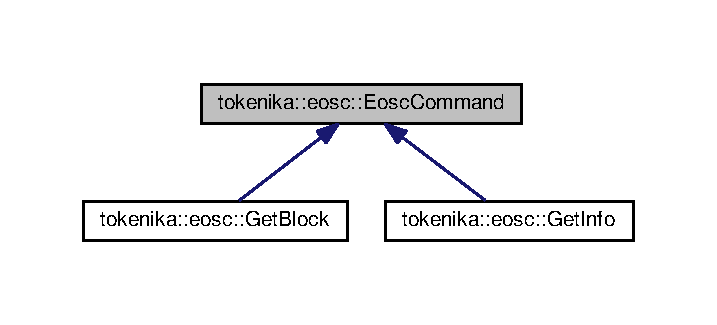
\includegraphics[width=344pt]{classtokenika_1_1eosc_1_1_eosc_command__inherit__graph}
\end{center}
\end{figure}
\subsection*{Public Member Functions}
\begin{DoxyCompactItemize}
\item 
\hyperlink{classtokenika_1_1eosc_1_1_eosc_command_ab736f0dcd8ca14eb0daf9b2244218397}{Eosc\+Command} (std\+::string path, boost\+::property\+\_\+tree\+::ptree post\+Json, bool is\+Raw=false)
\begin{DoxyCompactList}\small\item\em Initiates members, and calls the blockchain. \end{DoxyCompactList}\item 
bool \hyperlink{classtokenika_1_1eosc_1_1_eosc_command_a63f3adace3f84b59f64c5a54ca0c18dc}{is\+Error} () const
\begin{DoxyCompactList}\small\item\em Error flag. \end{DoxyCompactList}\item 
boost\+::property\+\_\+tree\+::ptree \hyperlink{classtokenika_1_1eosc_1_1_eosc_command_a2b451aefc95258d481cff16747fa1888}{get\+Rcv\+Json} () const
\begin{DoxyCompactList}\small\item\em Blockchain responce. \end{DoxyCompactList}\item 
std\+::string \hyperlink{classtokenika_1_1eosc_1_1_eosc_command_a1cb0362dceb5999e7e06078223b20d91}{to\+String\+Post} () const
\begin{DoxyCompactList}\small\item\em Post json string representation. \end{DoxyCompactList}\item 
std\+::string \hyperlink{classtokenika_1_1eosc_1_1_eosc_command_ad01ef46444d9d8bc708b5d18605c3903}{to\+String\+Rcv} () const
\begin{DoxyCompactList}\small\item\em Received json string representation. \end{DoxyCompactList}\item 
{\footnotesize template$<$typename Type $>$ }\\Type \hyperlink{classtokenika_1_1eosc_1_1_eosc_command_aa1da6eb23f52159afa4a15e767cd7d6f}{get} (const boost\+::property\+\_\+tree\+::ptree\+::path\+\_\+type \&path) const
\begin{DoxyCompactList}\small\item\em Returns a value of a path of the received json. \end{DoxyCompactList}\end{DoxyCompactItemize}
\subsection*{Static Public Attributes}
\begin{DoxyCompactItemize}
\item 
\mbox{\Hypertarget{classtokenika_1_1eosc_1_1_eosc_command_a82163846139ac5fd47ffe3cb68251d4e}\label{classtokenika_1_1eosc_1_1_eosc_command_a82163846139ac5fd47ffe3cb68251d4e}} 
static std\+::string {\bfseries host} = \char`\"{}\char`\"{}
\item 
\mbox{\Hypertarget{classtokenika_1_1eosc_1_1_eosc_command_a8a10e9cc90a957a70f40a63c37581452}\label{classtokenika_1_1eosc_1_1_eosc_command_a8a10e9cc90a957a70f40a63c37581452}} 
static std\+::string {\bfseries port} = \char`\"{}\char`\"{}
\item 
\mbox{\Hypertarget{classtokenika_1_1eosc_1_1_eosc_command_a59e21016dc35f824b680b45a4be4b2e0}\label{classtokenika_1_1eosc_1_1_eosc_command_a59e21016dc35f824b680b45a4be4b2e0}} 
static std\+::string {\bfseries wallet\+Host} = \char`\"{}\char`\"{}
\item 
\mbox{\Hypertarget{classtokenika_1_1eosc_1_1_eosc_command_abd597bd241a7b1f371d46c42dd8daa53}\label{classtokenika_1_1eosc_1_1_eosc_command_abd597bd241a7b1f371d46c42dd8daa53}} 
static std\+::string {\bfseries wallet\+Port} = \char`\"{}\char`\"{}
\item 
\mbox{\Hypertarget{classtokenika_1_1eosc_1_1_eosc_command_a32486030c8ca151b1492c124b6d380d0}\label{classtokenika_1_1eosc_1_1_eosc_command_a32486030c8ca151b1492c124b6d380d0}} 
static bool {\bfseries verbose} = false
\end{DoxyCompactItemize}
\subsection*{Protected Attributes}
\begin{DoxyCompactItemize}
\item 
\mbox{\Hypertarget{classtokenika_1_1eosc_1_1_eosc_command_a1642782c91f4877a8fba395324fb7337}\label{classtokenika_1_1eosc_1_1_eosc_command_a1642782c91f4877a8fba395324fb7337}} 
boost\+::property\+\_\+tree\+::ptree {\bfseries post\+Json}
\end{DoxyCompactItemize}


\subsection{Detailed Description}
Basic connection to the blockchain. 

Given a command path (for example {\ttfamily /v1/chain/\+Get\+Block}), and a json tree (for example \{\char`\"{}block\+\_\+num\+\_\+or\+\_\+id\char`\"{}=\char`\"{}25\char`\"{}\}), connects to the blockchain and receives a json reflacting an aspect of the blockchain state.

{\ttfamily \hyperlink{classtokenika_1_1eosc_1_1_eosc_command}{Eosc\+Command}} is the superclass for any specific command class in this library.

Parameters of the connection used are specified in file {\ttfamily eosc\+\_\+config.\+json}, in the root directory of the project. 

\subsection{Constructor \& Destructor Documentation}
\mbox{\Hypertarget{classtokenika_1_1eosc_1_1_eosc_command_ab736f0dcd8ca14eb0daf9b2244218397}\label{classtokenika_1_1eosc_1_1_eosc_command_ab736f0dcd8ca14eb0daf9b2244218397}} 
\index{tokenika\+::eosc\+::\+Eosc\+Command@{tokenika\+::eosc\+::\+Eosc\+Command}!Eosc\+Command@{Eosc\+Command}}
\index{Eosc\+Command@{Eosc\+Command}!tokenika\+::eosc\+::\+Eosc\+Command@{tokenika\+::eosc\+::\+Eosc\+Command}}
\subsubsection{\texorpdfstring{Eosc\+Command()}{EoscCommand()}}
{\footnotesize\ttfamily tokenika\+::eosc\+::\+Eosc\+Command\+::\+Eosc\+Command (\begin{DoxyParamCaption}\item[{std\+::string}]{path,  }\item[{boost\+::property\+\_\+tree\+::ptree}]{post\+Json,  }\item[{bool}]{is\+Raw = {\ttfamily false} }\end{DoxyParamCaption})}



Initiates members, and calls the blockchain. 


\begin{DoxyParams}{Parameters}
{\em path} & command path, for example {\ttfamily /v1/chain/\+Get\+Block} \\
\hline
{\em post\+Json} & json tree, for example \{\char`\"{}block\+\_\+num\+\_\+or\+\_\+id\char`\"{}=\char`\"{}25\char`\"{}\} \\
\hline
{\em is\+Raw} & boolean, determines printout of the to-\/string methods \\
\hline
\end{DoxyParams}


\subsection{Member Function Documentation}
\mbox{\Hypertarget{classtokenika_1_1eosc_1_1_eosc_command_aa1da6eb23f52159afa4a15e767cd7d6f}\label{classtokenika_1_1eosc_1_1_eosc_command_aa1da6eb23f52159afa4a15e767cd7d6f}} 
\index{tokenika\+::eosc\+::\+Eosc\+Command@{tokenika\+::eosc\+::\+Eosc\+Command}!get@{get}}
\index{get@{get}!tokenika\+::eosc\+::\+Eosc\+Command@{tokenika\+::eosc\+::\+Eosc\+Command}}
\subsubsection{\texorpdfstring{get()}{get()}}
{\footnotesize\ttfamily template$<$typename Type $>$ \\
Type tokenika\+::eosc\+::\+Eosc\+Command\+::get (\begin{DoxyParamCaption}\item[{const boost\+::property\+\_\+tree\+::ptree\+::path\+\_\+type \&}]{path }\end{DoxyParamCaption}) const\hspace{0.3cm}{\ttfamily [inline]}}



Returns a value of a path of the received json. 


\begin{DoxyTemplParams}{Template Parameters}
{\em Type} & type of the value \\
\hline
\end{DoxyTemplParams}

\begin{DoxyParams}{Parameters}
{\em path} & json tree path to the value \\
\hline
\end{DoxyParams}
\begin{DoxyReturn}{Returns}
Type the value of the given path 
\end{DoxyReturn}
\mbox{\Hypertarget{classtokenika_1_1eosc_1_1_eosc_command_a2b451aefc95258d481cff16747fa1888}\label{classtokenika_1_1eosc_1_1_eosc_command_a2b451aefc95258d481cff16747fa1888}} 
\index{tokenika\+::eosc\+::\+Eosc\+Command@{tokenika\+::eosc\+::\+Eosc\+Command}!get\+Rcv\+Json@{get\+Rcv\+Json}}
\index{get\+Rcv\+Json@{get\+Rcv\+Json}!tokenika\+::eosc\+::\+Eosc\+Command@{tokenika\+::eosc\+::\+Eosc\+Command}}
\subsubsection{\texorpdfstring{get\+Rcv\+Json()}{getRcvJson()}}
{\footnotesize\ttfamily boost\+::property\+\_\+tree\+::ptree tokenika\+::eosc\+::\+Eosc\+Command\+::get\+Rcv\+Json (\begin{DoxyParamCaption}{ }\end{DoxyParamCaption}) const\hspace{0.3cm}{\ttfamily [inline]}}



Blockchain responce. 

\begin{DoxyReturn}{Returns}
boost\+::property\+\_\+tree\+::ptree blockchain responce 
\end{DoxyReturn}
\mbox{\Hypertarget{classtokenika_1_1eosc_1_1_eosc_command_a63f3adace3f84b59f64c5a54ca0c18dc}\label{classtokenika_1_1eosc_1_1_eosc_command_a63f3adace3f84b59f64c5a54ca0c18dc}} 
\index{tokenika\+::eosc\+::\+Eosc\+Command@{tokenika\+::eosc\+::\+Eosc\+Command}!is\+Error@{is\+Error}}
\index{is\+Error@{is\+Error}!tokenika\+::eosc\+::\+Eosc\+Command@{tokenika\+::eosc\+::\+Eosc\+Command}}
\subsubsection{\texorpdfstring{is\+Error()}{isError()}}
{\footnotesize\ttfamily bool tokenika\+::eosc\+::\+Eosc\+Command\+::is\+Error (\begin{DoxyParamCaption}{ }\end{DoxyParamCaption}) const\hspace{0.3cm}{\ttfamily [inline]}}



Error flag. 

\begin{DoxyReturn}{Returns}
true if E\+OS blockchain responce is normal 

false if E\+OS blockchain responce is not normal 
\end{DoxyReturn}
\mbox{\Hypertarget{classtokenika_1_1eosc_1_1_eosc_command_a1cb0362dceb5999e7e06078223b20d91}\label{classtokenika_1_1eosc_1_1_eosc_command_a1cb0362dceb5999e7e06078223b20d91}} 
\index{tokenika\+::eosc\+::\+Eosc\+Command@{tokenika\+::eosc\+::\+Eosc\+Command}!to\+String\+Post@{to\+String\+Post}}
\index{to\+String\+Post@{to\+String\+Post}!tokenika\+::eosc\+::\+Eosc\+Command@{tokenika\+::eosc\+::\+Eosc\+Command}}
\subsubsection{\texorpdfstring{to\+String\+Post()}{toStringPost()}}
{\footnotesize\ttfamily std\+::string tokenika\+::eosc\+::\+Eosc\+Command\+::to\+String\+Post (\begin{DoxyParamCaption}{ }\end{DoxyParamCaption}) const}



Post json string representation. 

Returns post json string representation. I can be pretty or raw, depending ib the {\ttfamily is\+Raw} flag.

\begin{DoxyReturn}{Returns}
std\+::string post json string representation 
\end{DoxyReturn}
\mbox{\Hypertarget{classtokenika_1_1eosc_1_1_eosc_command_ad01ef46444d9d8bc708b5d18605c3903}\label{classtokenika_1_1eosc_1_1_eosc_command_ad01ef46444d9d8bc708b5d18605c3903}} 
\index{tokenika\+::eosc\+::\+Eosc\+Command@{tokenika\+::eosc\+::\+Eosc\+Command}!to\+String\+Rcv@{to\+String\+Rcv}}
\index{to\+String\+Rcv@{to\+String\+Rcv}!tokenika\+::eosc\+::\+Eosc\+Command@{tokenika\+::eosc\+::\+Eosc\+Command}}
\subsubsection{\texorpdfstring{to\+String\+Rcv()}{toStringRcv()}}
{\footnotesize\ttfamily std\+::string tokenika\+::eosc\+::\+Eosc\+Command\+::to\+String\+Rcv (\begin{DoxyParamCaption}{ }\end{DoxyParamCaption}) const}



Received json string representation. 

Returns received json string representation. I can be pretty or raw, depending ib the {\ttfamily is\+Raw} flag.

\begin{DoxyReturn}{Returns}
std\+::string received json string representation 
\end{DoxyReturn}


The documentation for this class was generated from the following files\+:\begin{DoxyCompactItemize}
\item 
\hyperlink{eosc__command_8hpp}{eosc\+\_\+command.\+hpp}\item 
eosc\+\_\+command.\+cpp\end{DoxyCompactItemize}

\hypertarget{classtokenika_1_1eosc_1_1_get_block}{}\section{tokenika\+:\+:eosc\+:\+:Get\+Block Class Reference}
\label{classtokenika_1_1eosc_1_1_get_block}\index{tokenika\+::eosc\+::\+Get\+Block@{tokenika\+::eosc\+::\+Get\+Block}}


Retrieve a full block from a blockchain.  




{\ttfamily \#include $<$eosc\+\_\+get\+\_\+commands.\+hpp$>$}



Inheritance diagram for tokenika\+:\+:eosc\+:\+:Get\+Block\+:\nopagebreak
\begin{figure}[H]
\begin{center}
\leavevmode
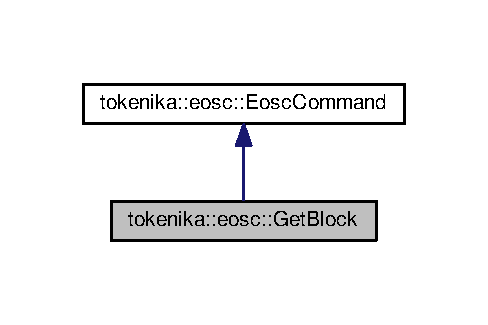
\includegraphics[width=234pt]{classtokenika_1_1eosc_1_1_get_block__inherit__graph}
\end{center}
\end{figure}


Collaboration diagram for tokenika\+:\+:eosc\+:\+:Get\+Block\+:\nopagebreak
\begin{figure}[H]
\begin{center}
\leavevmode
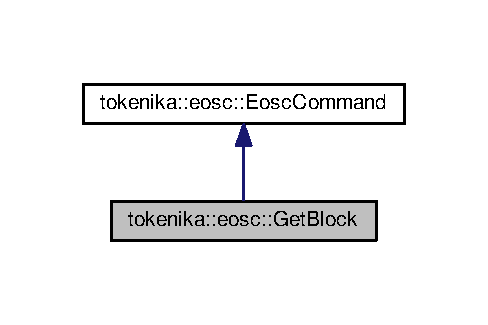
\includegraphics[width=234pt]{classtokenika_1_1eosc_1_1_get_block__coll__graph}
\end{center}
\end{figure}
\subsection*{Public Member Functions}
\begin{DoxyCompactItemize}
\item 
\mbox{\Hypertarget{classtokenika_1_1eosc_1_1_get_block_a67c1536e676f26b9e9dac915092f9627}\label{classtokenika_1_1eosc_1_1_get_block_a67c1536e676f26b9e9dac915092f9627}} 
{\bfseries Get\+Block} (boost\+::property\+\_\+tree\+::ptree post\+Json, bool raw=false)
\end{DoxyCompactItemize}
\subsection*{Additional Inherited Members}


\subsection{Detailed Description}
Retrieve a full block from a blockchain. 

Given a {\ttfamily boost\+::property\+\_\+tree\+::ptree json}, conforms (\href{#https://github.com/EOSIO/eosjs-json/blob/master/api/v1/chain.json}{\tt after eosjs-\/json}) this pattern\+: \begin{DoxyVerb}* {"block_num_or_id":"uint32 | string"}.
* \end{DoxyVerb}


the constructor posts it to an E\+OS block socket, specified in the {\ttfamily eosc\+\_\+config.\+json} file. The responce of the blockchain is, again, a {\ttfamily boost\+::property\+\_\+tree\+::ptree json}. On error, the reaponce json is {\ttfamily \{\char`\"{}error\char`\"{}\+:\char`\"{}error message\char`\"{}\}}, otherwise it conforms (\href{#https://github.com/EOSIO/eosjs-json/blob/master/api/v1/chain.json}{\tt after eosjs-\/json}) this pattern\+: \begin{DoxyVerb}* {
* "previous":"uint32",
* "timestamp":"2017-07-18T20:16:36",
* "transaction_merkle_root":"uint32",
* "producer":"uint16",
* "producer_changes":"map<account_name, account_name>[]",
* "producer_signature":"signature",
* "cycles":"thread[]",
* "id":"fixed_bytes33",
* "block_num":"uint32",
* "refBlockPrefix":"uint32"
* }
* \end{DoxyVerb}


It is available with the \hyperlink{classtokenika_1_1eosc_1_1_eosc_command_a2b451aefc95258d481cff16747fa1888}{tokenika\+::eosc\+::\+Eosc\+Command\+::get\+Rcv\+Json()} method.

Note that time is a string. For processing, it has to be expressed as a structure and afterwords back to a string. Helper functions, namely \+::str\+To\+Time(const std\+::string)

Example\+:

\begin{DoxyVerb}* #include <stdio.h>
* #include <stdlib.h>
* #include <iostream>
* #include <string>
*
* #include <boost/property_tree/ptree.hpp>
* #include "boost/date_time/posix_time/posix_time.hpp"
*
* #include "EoscCommands/eosc_get_commands.hpp"
*
* int main(int argc, char *argv[])
* {
* boost::property_tree::ptree postJson;
* postJson.put("block_num_or_id", 25);
* tokenika::eosc::GetBlock getBlock(getInfoPostJson);
* if(!getBlock.isError())
* {
*    std::cout << getBlock.get<int>("last_irreversible_block_num")) << std::endl;
*    boost::posix_time::ptime time = GetInfo.get<boost::posix_time::ptime>("timestamp");
*    std::cout << time << std::endl;
*    boost::posix_time::ptime t1 = time + boost::posix_time::seconds(900);
*    cout << (boost::posix_time::to_iso_extended_string)(t1) << endl;
* } else
* {
*    std::cerr << getBlock.get<string>("error")) << std::endl;
* }
*
* return 0;
* }
* \end{DoxyVerb}
 

The documentation for this class was generated from the following file\+:\begin{DoxyCompactItemize}
\item 
\hyperlink{eosc__get__commands_8hpp}{eosc\+\_\+get\+\_\+commands.\+hpp}\end{DoxyCompactItemize}

\hypertarget{classtokenika_1_1eosc_1_1_get_block_options}{}\section{tokenika\+:\+:eosc\+:\+:Get\+Block\+Options Class Reference}
\label{classtokenika_1_1eosc_1_1_get_block_options}\index{tokenika\+::eosc\+::\+Get\+Block\+Options@{tokenika\+::eosc\+::\+Get\+Block\+Options}}


Inheritance diagram for tokenika\+:\+:eosc\+:\+:Get\+Block\+Options\+:\nopagebreak
\begin{figure}[H]
\begin{center}
\leavevmode
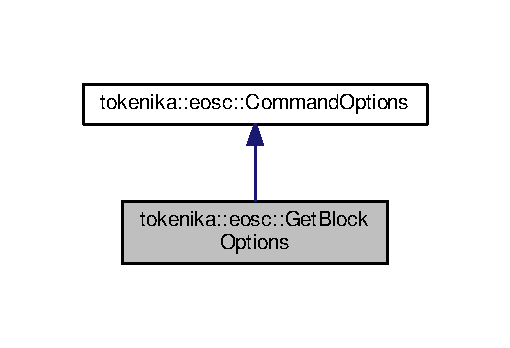
\includegraphics[width=245pt]{classtokenika_1_1eosc_1_1_get_block_options__inherit__graph}
\end{center}
\end{figure}


Collaboration diagram for tokenika\+:\+:eosc\+:\+:Get\+Block\+Options\+:\nopagebreak
\begin{figure}[H]
\begin{center}
\leavevmode
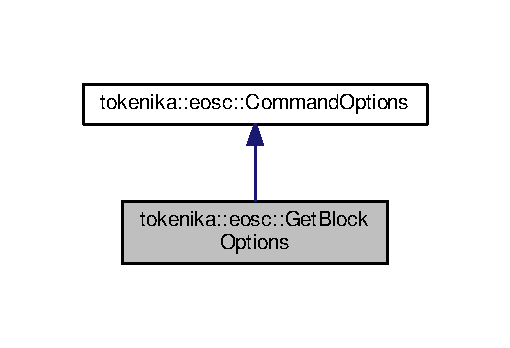
\includegraphics[width=245pt]{classtokenika_1_1eosc_1_1_get_block_options__coll__graph}
\end{center}
\end{figure}
\subsection*{Public Member Functions}
\begin{DoxyCompactItemize}
\item 
\mbox{\Hypertarget{classtokenika_1_1eosc_1_1_get_block_options_ab031795a5bd5cf681307cc9ea07659a3}\label{classtokenika_1_1eosc_1_1_get_block_options_ab031795a5bd5cf681307cc9ea07659a3}} 
{\bfseries Get\+Block\+Options} (int argc, const char $\ast$$\ast$argv)
\end{DoxyCompactItemize}
\subsection*{Protected Member Functions}
\begin{DoxyCompactItemize}
\item 
const char $\ast$ \hyperlink{classtokenika_1_1eosc_1_1_get_block_options_ab0b7572223d35a3232630b9eef51b9cb}{get\+Usage} ()
\begin{DoxyCompactList}\small\item\em Command \textquotesingle{}usage\textquotesingle{} instruction. \end{DoxyCompactList}\item 
virtual boost\+::program\+\_\+options\+::options\+\_\+description \hyperlink{classtokenika_1_1eosc_1_1_get_block_options_a6e8c1a240e5a529c093e0053f12e9ee5}{options} ()
\begin{DoxyCompactList}\small\item\em List of the command options. \end{DoxyCompactList}\item 
virtual void \hyperlink{classtokenika_1_1eosc_1_1_get_block_options_ac6f55ff885c6a553a16ee0b09a0d9da1}{set\+Pos\+Desc} (boost\+::program\+\_\+options\+::positional\+\_\+options\+\_\+description \&pos\+\_\+desc)
\begin{DoxyCompactList}\small\item\em Positional options. \end{DoxyCompactList}\item 
virtual bool \hyperlink{classtokenika_1_1eosc_1_1_get_block_options_a71450327dcf082d00f4c3e3b5c43e619}{set\+Json} (boost\+::program\+\_\+options\+::variables\+\_\+map \&vm)
\begin{DoxyCompactList}\small\item\em Fills the post json tree according to options. \end{DoxyCompactList}\item 
virtual \hyperlink{classtokenika_1_1eosc_1_1_eosc_command}{Eosc\+Command} \hyperlink{classtokenika_1_1eosc_1_1_get_block_options_ac1c5b62f162c4253cab8de5a93fe5cf9}{get\+Command} (bool is\+\_\+raw)
\begin{DoxyCompactList}\small\item\em Returns command object, containing a responce frosource /mnt/hgfs/\+Workspaces/\+E\+O\+S/eosc\+Bash/eosc\+Bash \$\+E\+O\+S\+I\+O\+\_\+\+I\+N\+S\+T\+A\+L\+L\+\_\+\+D\+IR m the blockchain. \end{DoxyCompactList}\item 
virtual void \hyperlink{classtokenika_1_1eosc_1_1_get_block_options_a8d45be43c2a93468910db4533db832cc}{get\+Output} (\hyperlink{classtokenika_1_1eosc_1_1_eosc_command}{Eosc\+Command} command)
\begin{DoxyCompactList}\small\item\em Placeholder for printout instructions. \end{DoxyCompactList}\item 
virtual void \hyperlink{classtokenika_1_1eosc_1_1_get_block_options_ace1d886b5fb260150df8d291339fbd03}{get\+Example} ()
\begin{DoxyCompactList}\small\item\em Placeholder for any exemplary code snippet. \end{DoxyCompactList}\end{DoxyCompactItemize}
\subsection*{Protected Attributes}
\begin{DoxyCompactItemize}
\item 
\mbox{\Hypertarget{classtokenika_1_1eosc_1_1_get_block_options_af6c20effd6a52b8d26a8377450585142}\label{classtokenika_1_1eosc_1_1_get_block_options_af6c20effd6a52b8d26a8377450585142}} 
int {\bfseries n}
\item 
\mbox{\Hypertarget{classtokenika_1_1eosc_1_1_get_block_options_a0eda5e812218067adfc5bbab2d6b4048}\label{classtokenika_1_1eosc_1_1_get_block_options_a0eda5e812218067adfc5bbab2d6b4048}} 
std\+::string {\bfseries id}
\end{DoxyCompactItemize}


\subsection{Member Function Documentation}
\mbox{\Hypertarget{classtokenika_1_1eosc_1_1_get_block_options_ac1c5b62f162c4253cab8de5a93fe5cf9}\label{classtokenika_1_1eosc_1_1_get_block_options_ac1c5b62f162c4253cab8de5a93fe5cf9}} 
\index{tokenika\+::eosc\+::\+Get\+Block\+Options@{tokenika\+::eosc\+::\+Get\+Block\+Options}!get\+Command@{get\+Command}}
\index{get\+Command@{get\+Command}!tokenika\+::eosc\+::\+Get\+Block\+Options@{tokenika\+::eosc\+::\+Get\+Block\+Options}}
\subsubsection{\texorpdfstring{get\+Command()}{getCommand()}}
{\footnotesize\ttfamily virtual \hyperlink{classtokenika_1_1eosc_1_1_eosc_command}{Eosc\+Command} tokenika\+::eosc\+::\+Get\+Block\+Options\+::get\+Command (\begin{DoxyParamCaption}\item[{bool}]{is\+Raw }\end{DoxyParamCaption})\hspace{0.3cm}{\ttfamily [inline]}, {\ttfamily [protected]}, {\ttfamily [virtual]}}



Returns command object, containing a responce frosource /mnt/hgfs/\+Workspaces/\+E\+O\+S/eosc\+Bash/eosc\+Bash \$\+E\+O\+S\+I\+O\+\_\+\+I\+N\+S\+T\+A\+L\+L\+\_\+\+D\+IR m the blockchain. 


\begin{DoxyParams}{Parameters}
{\em is\+Raw} & raw or pretty printout flag \\
\hline
\end{DoxyParams}
\begin{DoxyReturn}{Returns}
\hyperlink{classtokenika_1_1eosc_1_1_eosc_command}{Eosc\+Command} command object 
\end{DoxyReturn}


Reimplemented from \hyperlink{classtokenika_1_1eosc_1_1_command_options_a787f15164e2055394d9d948c07bf201c}{tokenika\+::eosc\+::\+Command\+Options}.

\mbox{\Hypertarget{classtokenika_1_1eosc_1_1_get_block_options_ace1d886b5fb260150df8d291339fbd03}\label{classtokenika_1_1eosc_1_1_get_block_options_ace1d886b5fb260150df8d291339fbd03}} 
\index{tokenika\+::eosc\+::\+Get\+Block\+Options@{tokenika\+::eosc\+::\+Get\+Block\+Options}!get\+Example@{get\+Example}}
\index{get\+Example@{get\+Example}!tokenika\+::eosc\+::\+Get\+Block\+Options@{tokenika\+::eosc\+::\+Get\+Block\+Options}}
\subsubsection{\texorpdfstring{get\+Example()}{getExample()}}
{\footnotesize\ttfamily virtual void tokenika\+::eosc\+::\+Get\+Block\+Options\+::get\+Example (\begin{DoxyParamCaption}{ }\end{DoxyParamCaption})\hspace{0.3cm}{\ttfamily [inline]}, {\ttfamily [protected]}, {\ttfamily [virtual]}}



Placeholder for any exemplary code snippet. 

source /mnt/hgfs/\+Workspaces/\+E\+O\+S/eosc\+Bash/eosc\+Bash \$\+E\+O\+S\+I\+O\+\_\+\+I\+N\+S\+T\+A\+L\+L\+\_\+\+D\+IR 

Reimplemented from \hyperlink{classtokenika_1_1eosc_1_1_command_options_ab1fe134b6c2230257a5c07b021812986}{tokenika\+::eosc\+::\+Command\+Options}.

\mbox{\Hypertarget{classtokenika_1_1eosc_1_1_get_block_options_a8d45be43c2a93468910db4533db832cc}\label{classtokenika_1_1eosc_1_1_get_block_options_a8d45be43c2a93468910db4533db832cc}} 
\index{tokenika\+::eosc\+::\+Get\+Block\+Options@{tokenika\+::eosc\+::\+Get\+Block\+Options}!get\+Output@{get\+Output}}
\index{get\+Output@{get\+Output}!tokenika\+::eosc\+::\+Get\+Block\+Options@{tokenika\+::eosc\+::\+Get\+Block\+Options}}
\subsubsection{\texorpdfstring{get\+Output()}{getOutput()}}
{\footnotesize\ttfamily virtual void tokenika\+::eosc\+::\+Get\+Block\+Options\+::get\+Output (\begin{DoxyParamCaption}\item[{\hyperlink{classtokenika_1_1eosc_1_1_eosc_command}{Eosc\+Command}}]{command }\end{DoxyParamCaption})\hspace{0.3cm}{\ttfamily [inline]}, {\ttfamily [protected]}, {\ttfamily [virtual]}}



Placeholder for printout instructions. 

Placeholder for printout instructions. Printout should be composed with the \+::output(const char$\ast$, const char$\ast$, ...) function.


\begin{DoxyParams}{Parameters}
{\em command} & command object, containing a responce from the blockchain. \\
\hline
\end{DoxyParams}


Reimplemented from \hyperlink{classtokenika_1_1eosc_1_1_command_options_a346dcfb00b8ac522169714544bfa7be0}{tokenika\+::eosc\+::\+Command\+Options}.

\mbox{\Hypertarget{classtokenika_1_1eosc_1_1_get_block_options_ab0b7572223d35a3232630b9eef51b9cb}\label{classtokenika_1_1eosc_1_1_get_block_options_ab0b7572223d35a3232630b9eef51b9cb}} 
\index{tokenika\+::eosc\+::\+Get\+Block\+Options@{tokenika\+::eosc\+::\+Get\+Block\+Options}!get\+Usage@{get\+Usage}}
\index{get\+Usage@{get\+Usage}!tokenika\+::eosc\+::\+Get\+Block\+Options@{tokenika\+::eosc\+::\+Get\+Block\+Options}}
\subsubsection{\texorpdfstring{get\+Usage()}{getUsage()}}
{\footnotesize\ttfamily const char$\ast$ tokenika\+::eosc\+::\+Get\+Block\+Options\+::get\+Usage (\begin{DoxyParamCaption}{ }\end{DoxyParamCaption})\hspace{0.3cm}{\ttfamily [inline]}, {\ttfamily [protected]}, {\ttfamily [virtual]}}



Command \textquotesingle{}usage\textquotesingle{} instruction. 

\begin{DoxyReturn}{Returns}
const char$\ast$ usage text 
\end{DoxyReturn}


Reimplemented from \hyperlink{classtokenika_1_1eosc_1_1_command_options_a18ada0ba1163f7a41c9990ae2756012b}{tokenika\+::eosc\+::\+Command\+Options}.

\mbox{\Hypertarget{classtokenika_1_1eosc_1_1_get_block_options_a6e8c1a240e5a529c093e0053f12e9ee5}\label{classtokenika_1_1eosc_1_1_get_block_options_a6e8c1a240e5a529c093e0053f12e9ee5}} 
\index{tokenika\+::eosc\+::\+Get\+Block\+Options@{tokenika\+::eosc\+::\+Get\+Block\+Options}!options@{options}}
\index{options@{options}!tokenika\+::eosc\+::\+Get\+Block\+Options@{tokenika\+::eosc\+::\+Get\+Block\+Options}}
\subsubsection{\texorpdfstring{options()}{options()}}
{\footnotesize\ttfamily virtual boost\+::program\+\_\+options\+::options\+\_\+description tokenika\+::eosc\+::\+Get\+Block\+Options\+::options (\begin{DoxyParamCaption}{ }\end{DoxyParamCaption})\hspace{0.3cm}{\ttfamily [inline]}, {\ttfamily [protected]}, {\ttfamily [virtual]}}



List of the command options. 

\begin{DoxyReturn}{Returns}
boost\+::program\+\_\+options\+::options\+\_\+description command options 
\end{DoxyReturn}


Reimplemented from \hyperlink{classtokenika_1_1eosc_1_1_command_options_aa55960f380250eb7065cb6489b67196f}{tokenika\+::eosc\+::\+Command\+Options}.

\mbox{\Hypertarget{classtokenika_1_1eosc_1_1_get_block_options_a71450327dcf082d00f4c3e3b5c43e619}\label{classtokenika_1_1eosc_1_1_get_block_options_a71450327dcf082d00f4c3e3b5c43e619}} 
\index{tokenika\+::eosc\+::\+Get\+Block\+Options@{tokenika\+::eosc\+::\+Get\+Block\+Options}!set\+Json@{set\+Json}}
\index{set\+Json@{set\+Json}!tokenika\+::eosc\+::\+Get\+Block\+Options@{tokenika\+::eosc\+::\+Get\+Block\+Options}}
\subsubsection{\texorpdfstring{set\+Json()}{setJson()}}
{\footnotesize\ttfamily virtual bool tokenika\+::eosc\+::\+Get\+Block\+Options\+::set\+Json (\begin{DoxyParamCaption}\item[{boost\+::program\+\_\+options\+::variables\+\_\+map \&}]{vm }\end{DoxyParamCaption})\hspace{0.3cm}{\ttfamily [inline]}, {\ttfamily [protected]}, {\ttfamily [virtual]}}



Fills the post json tree according to options. 


\begin{DoxyParams}{Parameters}
{\em vm} & boost program options variable map \\
\hline
\end{DoxyParams}
\begin{DoxyReturn}{Returns}
true if post json is set completely 

false if post json cannot be set completely 
\end{DoxyReturn}


Reimplemented from \hyperlink{classtokenika_1_1eosc_1_1_command_options_a7aecc9aa79ca65f6abbd568ff8ff77a7}{tokenika\+::eosc\+::\+Command\+Options}.

\mbox{\Hypertarget{classtokenika_1_1eosc_1_1_get_block_options_ac6f55ff885c6a553a16ee0b09a0d9da1}\label{classtokenika_1_1eosc_1_1_get_block_options_ac6f55ff885c6a553a16ee0b09a0d9da1}} 
\index{tokenika\+::eosc\+::\+Get\+Block\+Options@{tokenika\+::eosc\+::\+Get\+Block\+Options}!set\+Pos\+Desc@{set\+Pos\+Desc}}
\index{set\+Pos\+Desc@{set\+Pos\+Desc}!tokenika\+::eosc\+::\+Get\+Block\+Options@{tokenika\+::eosc\+::\+Get\+Block\+Options}}
\subsubsection{\texorpdfstring{set\+Pos\+Desc()}{setPosDesc()}}
{\footnotesize\ttfamily virtual void tokenika\+::eosc\+::\+Get\+Block\+Options\+::set\+Pos\+Desc (\begin{DoxyParamCaption}\item[{boost\+::program\+\_\+options\+::positional\+\_\+options\+\_\+description \&}]{pos\+\_\+descr }\end{DoxyParamCaption})\hspace{0.3cm}{\ttfamily [inline]}, {\ttfamily [protected]}, {\ttfamily [virtual]}}



Positional options. 


\begin{DoxyParams}{Parameters}
{\em pos\+\_\+descr} & positional options \\
\hline
\end{DoxyParams}


Reimplemented from \hyperlink{classtokenika_1_1eosc_1_1_command_options_ae2e98c683ae1eb3e5af1e81e60020447}{tokenika\+::eosc\+::\+Command\+Options}.



The documentation for this class was generated from the following file\+:\begin{DoxyCompactItemize}
\item 
\hyperlink{eosc__get__commands_8hpp}{eosc\+\_\+get\+\_\+commands.\+hpp}\end{DoxyCompactItemize}

\hypertarget{classtokenika_1_1eosc_1_1_get_info}{}\section{tokenika\+:\+:eosc\+:\+:Get\+Info Class Reference}
\label{classtokenika_1_1eosc_1_1_get_info}\index{tokenika\+::eosc\+::\+Get\+Info@{tokenika\+::eosc\+::\+Get\+Info}}


Get current blockchain information.  




{\ttfamily \#include $<$eosc\+\_\+get\+\_\+commands.\+hpp$>$}



Inheritance diagram for tokenika\+:\+:eosc\+:\+:Get\+Info\+:\nopagebreak
\begin{figure}[H]
\begin{center}
\leavevmode
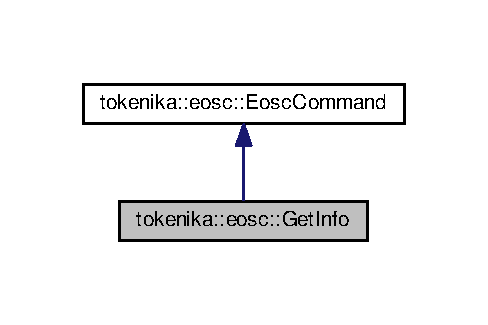
\includegraphics[width=234pt]{classtokenika_1_1eosc_1_1_get_info__inherit__graph}
\end{center}
\end{figure}


Collaboration diagram for tokenika\+:\+:eosc\+:\+:Get\+Info\+:\nopagebreak
\begin{figure}[H]
\begin{center}
\leavevmode
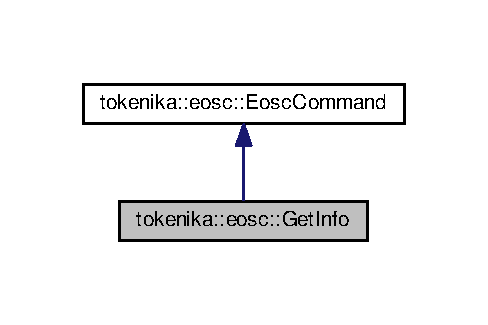
\includegraphics[width=234pt]{classtokenika_1_1eosc_1_1_get_info__coll__graph}
\end{center}
\end{figure}
\subsection*{Public Member Functions}
\begin{DoxyCompactItemize}
\item 
\mbox{\Hypertarget{classtokenika_1_1eosc_1_1_get_info_a3b219ff2f0036acbecf97922e28c3793}\label{classtokenika_1_1eosc_1_1_get_info_a3b219ff2f0036acbecf97922e28c3793}} 
{\bfseries Get\+Info} (boost\+::property\+\_\+tree\+::ptree post\+Json, bool raw=false)
\end{DoxyCompactItemize}
\subsection*{Additional Inherited Members}


\subsection{Detailed Description}
Get current blockchain information. 

Example\+:

\begin{DoxyVerb}* #include <stdio.h>
* #include <stdlib.h>
* #include <iostream>
* #include <string>
* #include <boost/property_tree/ptree.hpp>
* #include "EoscCommands/eosc_get_commands.hpp"
*
* int main(int argc, char *argv[])
* {
* boost::property_tree::ptree postJson;
* tokenika::eosc::GetInfo GetInfo(getInfoPostJson);
* std::cout << GetInfo.get<int>("last_irreversible_block_num")) << std::endl;
* boost::property_tree::ptree rcv_json = GetInfo.getRcvJson();
* std::cout << GetBlock.toStringRcv() << std::endl; // Print the response json.
*
* return 0;
* }
* \end{DoxyVerb}
 

The documentation for this class was generated from the following file\+:\begin{DoxyCompactItemize}
\item 
\hyperlink{eosc__get__commands_8hpp}{eosc\+\_\+get\+\_\+commands.\+hpp}\end{DoxyCompactItemize}

\hypertarget{classtokenika_1_1eosc_1_1_get_info_options}{}\section{tokenika\+:\+:eosc\+:\+:Get\+Info\+Options Class Reference}
\label{classtokenika_1_1eosc_1_1_get_info_options}\index{tokenika\+::eosc\+::\+Get\+Info\+Options@{tokenika\+::eosc\+::\+Get\+Info\+Options}}


Inheritance diagram for tokenika\+:\+:eosc\+:\+:Get\+Info\+Options\+:\nopagebreak
\begin{figure}[H]
\begin{center}
\leavevmode
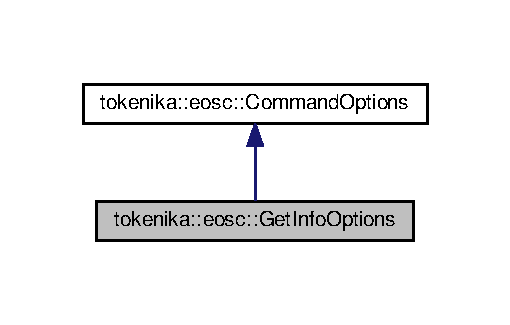
\includegraphics[width=245pt]{classtokenika_1_1eosc_1_1_get_info_options__inherit__graph}
\end{center}
\end{figure}


Collaboration diagram for tokenika\+:\+:eosc\+:\+:Get\+Info\+Options\+:\nopagebreak
\begin{figure}[H]
\begin{center}
\leavevmode
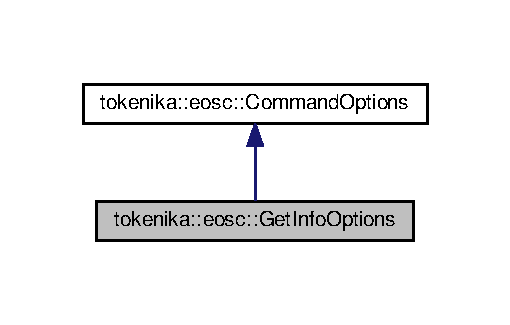
\includegraphics[width=245pt]{classtokenika_1_1eosc_1_1_get_info_options__coll__graph}
\end{center}
\end{figure}
\subsection*{Public Member Functions}
\begin{DoxyCompactItemize}
\item 
\mbox{\Hypertarget{classtokenika_1_1eosc_1_1_get_info_options_a9d3325947476e5eb6f3a44ebd28c02d8}\label{classtokenika_1_1eosc_1_1_get_info_options_a9d3325947476e5eb6f3a44ebd28c02d8}} 
{\bfseries Get\+Info\+Options} (int argc, const char $\ast$$\ast$argv)
\end{DoxyCompactItemize}
\subsection*{Protected Member Functions}
\begin{DoxyCompactItemize}
\item 
const char $\ast$ \hyperlink{classtokenika_1_1eosc_1_1_get_info_options_aad995529f121f42cdd8f0b1380540370}{get\+Usage} ()
\begin{DoxyCompactList}\small\item\em Command \textquotesingle{}usage\textquotesingle{} instruction. \end{DoxyCompactList}\item 
virtual bool \hyperlink{classtokenika_1_1eosc_1_1_get_info_options_a15688c1262b3d861bd7de015e92dd6a7}{set\+Json} (boost\+::program\+\_\+options\+::variables\+\_\+map \&vm)
\begin{DoxyCompactList}\small\item\em Fills the post json tree according to options. \end{DoxyCompactList}\item 
virtual \hyperlink{classtokenika_1_1eosc_1_1_eosc_command}{Eosc\+Command} \hyperlink{classtokenika_1_1eosc_1_1_get_info_options_a7283bdc9a328ccd8a29a25bcdc01dfa6}{get\+Command} (bool is\+\_\+raw)
\begin{DoxyCompactList}\small\item\em Returns command object, containing a responce frosource /mnt/hgfs/\+Workspaces/\+E\+O\+S/eosc\+Bash/eosc\+Bash \$\+E\+O\+S\+I\+O\+\_\+\+I\+N\+S\+T\+A\+L\+L\+\_\+\+D\+IR m the blockchain. \end{DoxyCompactList}\item 
virtual void \hyperlink{classtokenika_1_1eosc_1_1_get_info_options_a73ebf397cd94b45513f1e049cbbb0eb5}{get\+Output} (\hyperlink{classtokenika_1_1eosc_1_1_eosc_command}{tokenika\+::eosc\+::\+Eosc\+Command} command)
\begin{DoxyCompactList}\small\item\em Placeholder for printout instructions. \end{DoxyCompactList}\item 
virtual void \hyperlink{classtokenika_1_1eosc_1_1_get_info_options_a652a64ac80195f98b33ae91a2b284316}{get\+Example} ()
\begin{DoxyCompactList}\small\item\em Placeholder for any exemplary code snippet. \end{DoxyCompactList}\end{DoxyCompactItemize}
\subsection*{Additional Inherited Members}


\subsection{Member Function Documentation}
\mbox{\Hypertarget{classtokenika_1_1eosc_1_1_get_info_options_a7283bdc9a328ccd8a29a25bcdc01dfa6}\label{classtokenika_1_1eosc_1_1_get_info_options_a7283bdc9a328ccd8a29a25bcdc01dfa6}} 
\index{tokenika\+::eosc\+::\+Get\+Info\+Options@{tokenika\+::eosc\+::\+Get\+Info\+Options}!get\+Command@{get\+Command}}
\index{get\+Command@{get\+Command}!tokenika\+::eosc\+::\+Get\+Info\+Options@{tokenika\+::eosc\+::\+Get\+Info\+Options}}
\subsubsection{\texorpdfstring{get\+Command()}{getCommand()}}
{\footnotesize\ttfamily virtual \hyperlink{classtokenika_1_1eosc_1_1_eosc_command}{Eosc\+Command} tokenika\+::eosc\+::\+Get\+Info\+Options\+::get\+Command (\begin{DoxyParamCaption}\item[{bool}]{is\+Raw }\end{DoxyParamCaption})\hspace{0.3cm}{\ttfamily [inline]}, {\ttfamily [protected]}, {\ttfamily [virtual]}}



Returns command object, containing a responce frosource /mnt/hgfs/\+Workspaces/\+E\+O\+S/eosc\+Bash/eosc\+Bash \$\+E\+O\+S\+I\+O\+\_\+\+I\+N\+S\+T\+A\+L\+L\+\_\+\+D\+IR m the blockchain. 


\begin{DoxyParams}{Parameters}
{\em is\+Raw} & raw or pretty printout flag \\
\hline
\end{DoxyParams}
\begin{DoxyReturn}{Returns}
\hyperlink{classtokenika_1_1eosc_1_1_eosc_command}{Eosc\+Command} command object 
\end{DoxyReturn}


Reimplemented from \hyperlink{classtokenika_1_1eosc_1_1_command_options_a787f15164e2055394d9d948c07bf201c}{tokenika\+::eosc\+::\+Command\+Options}.

\mbox{\Hypertarget{classtokenika_1_1eosc_1_1_get_info_options_a652a64ac80195f98b33ae91a2b284316}\label{classtokenika_1_1eosc_1_1_get_info_options_a652a64ac80195f98b33ae91a2b284316}} 
\index{tokenika\+::eosc\+::\+Get\+Info\+Options@{tokenika\+::eosc\+::\+Get\+Info\+Options}!get\+Example@{get\+Example}}
\index{get\+Example@{get\+Example}!tokenika\+::eosc\+::\+Get\+Info\+Options@{tokenika\+::eosc\+::\+Get\+Info\+Options}}
\subsubsection{\texorpdfstring{get\+Example()}{getExample()}}
{\footnotesize\ttfamily virtual void tokenika\+::eosc\+::\+Get\+Info\+Options\+::get\+Example (\begin{DoxyParamCaption}{ }\end{DoxyParamCaption})\hspace{0.3cm}{\ttfamily [inline]}, {\ttfamily [protected]}, {\ttfamily [virtual]}}



Placeholder for any exemplary code snippet. 

source /mnt/hgfs/\+Workspaces/\+E\+O\+S/eosc\+Bash/eosc\+Bash \$\+E\+O\+S\+I\+O\+\_\+\+I\+N\+S\+T\+A\+L\+L\+\_\+\+D\+IR 

Reimplemented from \hyperlink{classtokenika_1_1eosc_1_1_command_options_ab1fe134b6c2230257a5c07b021812986}{tokenika\+::eosc\+::\+Command\+Options}.

\mbox{\Hypertarget{classtokenika_1_1eosc_1_1_get_info_options_a73ebf397cd94b45513f1e049cbbb0eb5}\label{classtokenika_1_1eosc_1_1_get_info_options_a73ebf397cd94b45513f1e049cbbb0eb5}} 
\index{tokenika\+::eosc\+::\+Get\+Info\+Options@{tokenika\+::eosc\+::\+Get\+Info\+Options}!get\+Output@{get\+Output}}
\index{get\+Output@{get\+Output}!tokenika\+::eosc\+::\+Get\+Info\+Options@{tokenika\+::eosc\+::\+Get\+Info\+Options}}
\subsubsection{\texorpdfstring{get\+Output()}{getOutput()}}
{\footnotesize\ttfamily virtual void tokenika\+::eosc\+::\+Get\+Info\+Options\+::get\+Output (\begin{DoxyParamCaption}\item[{\hyperlink{classtokenika_1_1eosc_1_1_eosc_command}{tokenika\+::eosc\+::\+Eosc\+Command}}]{command }\end{DoxyParamCaption})\hspace{0.3cm}{\ttfamily [inline]}, {\ttfamily [protected]}, {\ttfamily [virtual]}}



Placeholder for printout instructions. 

Placeholder for printout instructions. Printout should be composed with the \+::output(const char$\ast$, const char$\ast$, ...) function.


\begin{DoxyParams}{Parameters}
{\em command} & command object, containing a responce from the blockchain. \\
\hline
\end{DoxyParams}


Reimplemented from \hyperlink{classtokenika_1_1eosc_1_1_command_options_a346dcfb00b8ac522169714544bfa7be0}{tokenika\+::eosc\+::\+Command\+Options}.

\mbox{\Hypertarget{classtokenika_1_1eosc_1_1_get_info_options_aad995529f121f42cdd8f0b1380540370}\label{classtokenika_1_1eosc_1_1_get_info_options_aad995529f121f42cdd8f0b1380540370}} 
\index{tokenika\+::eosc\+::\+Get\+Info\+Options@{tokenika\+::eosc\+::\+Get\+Info\+Options}!get\+Usage@{get\+Usage}}
\index{get\+Usage@{get\+Usage}!tokenika\+::eosc\+::\+Get\+Info\+Options@{tokenika\+::eosc\+::\+Get\+Info\+Options}}
\subsubsection{\texorpdfstring{get\+Usage()}{getUsage()}}
{\footnotesize\ttfamily const char$\ast$ tokenika\+::eosc\+::\+Get\+Info\+Options\+::get\+Usage (\begin{DoxyParamCaption}{ }\end{DoxyParamCaption})\hspace{0.3cm}{\ttfamily [inline]}, {\ttfamily [protected]}, {\ttfamily [virtual]}}



Command \textquotesingle{}usage\textquotesingle{} instruction. 

\begin{DoxyReturn}{Returns}
const char$\ast$ usage text 
\end{DoxyReturn}


Reimplemented from \hyperlink{classtokenika_1_1eosc_1_1_command_options_a18ada0ba1163f7a41c9990ae2756012b}{tokenika\+::eosc\+::\+Command\+Options}.

\mbox{\Hypertarget{classtokenika_1_1eosc_1_1_get_info_options_a15688c1262b3d861bd7de015e92dd6a7}\label{classtokenika_1_1eosc_1_1_get_info_options_a15688c1262b3d861bd7de015e92dd6a7}} 
\index{tokenika\+::eosc\+::\+Get\+Info\+Options@{tokenika\+::eosc\+::\+Get\+Info\+Options}!set\+Json@{set\+Json}}
\index{set\+Json@{set\+Json}!tokenika\+::eosc\+::\+Get\+Info\+Options@{tokenika\+::eosc\+::\+Get\+Info\+Options}}
\subsubsection{\texorpdfstring{set\+Json()}{setJson()}}
{\footnotesize\ttfamily virtual bool tokenika\+::eosc\+::\+Get\+Info\+Options\+::set\+Json (\begin{DoxyParamCaption}\item[{boost\+::program\+\_\+options\+::variables\+\_\+map \&}]{vm }\end{DoxyParamCaption})\hspace{0.3cm}{\ttfamily [inline]}, {\ttfamily [protected]}, {\ttfamily [virtual]}}



Fills the post json tree according to options. 


\begin{DoxyParams}{Parameters}
{\em vm} & boost program options variable map \\
\hline
\end{DoxyParams}
\begin{DoxyReturn}{Returns}
true if post json is set completely 

false if post json cannot be set completely 
\end{DoxyReturn}


Reimplemented from \hyperlink{classtokenika_1_1eosc_1_1_command_options_a7aecc9aa79ca65f6abbd568ff8ff77a7}{tokenika\+::eosc\+::\+Command\+Options}.



The documentation for this class was generated from the following file\+:\begin{DoxyCompactItemize}
\item 
\hyperlink{eosc__get__commands_8hpp}{eosc\+\_\+get\+\_\+commands.\+hpp}\end{DoxyCompactItemize}

\hypertarget{structtokenika_1_1eosc_1_1_init_get_json}{}\section{tokenika\+:\+:eosc\+:\+:Init\+Get\+Json Struct Reference}
\label{structtokenika_1_1eosc_1_1_init_get_json}\index{tokenika\+::eosc\+::\+Init\+Get\+Json@{tokenika\+::eosc\+::\+Init\+Get\+Json}}
\subsection*{Data Fields}
\begin{DoxyCompactItemize}
\item 
\mbox{\Hypertarget{structtokenika_1_1eosc_1_1_init_get_json_a19564069824531cdead743209c1092e3}\label{structtokenika_1_1eosc_1_1_init_get_json_a19564069824531cdead743209c1092e3}} 
std\+::string {\bfseries str\+Val}
\item 
\mbox{\Hypertarget{structtokenika_1_1eosc_1_1_init_get_json_a39b17a82f0b5c2346756683665594a39}\label{structtokenika_1_1eosc_1_1_init_get_json_a39b17a82f0b5c2346756683665594a39}} 
int {\bfseries int\+Val}
\item 
\mbox{\Hypertarget{structtokenika_1_1eosc_1_1_init_get_json_a2bd646a37a513d5a49e2e8a6bcfa6c43}\label{structtokenika_1_1eosc_1_1_init_get_json_a2bd646a37a513d5a49e2e8a6bcfa6c43}} 
float {\bfseries float\+Val}
\item 
\mbox{\Hypertarget{structtokenika_1_1eosc_1_1_init_get_json_ad7763c3fb45c04c17c292e00220e4ef9}\label{structtokenika_1_1eosc_1_1_init_get_json_ad7763c3fb45c04c17c292e00220e4ef9}} 
boost\+::posix\+\_\+time\+::ptime {\bfseries ptime}
\end{DoxyCompactItemize}


The documentation for this struct was generated from the following file\+:\begin{DoxyCompactItemize}
\item 
eosc\+\_\+command.\+cpp\end{DoxyCompactItemize}

\hypertarget{classserver}{}\section{server Class Reference}
\label{classserver}\index{server@{server}}
\subsection*{Public Member Functions}
\begin{DoxyCompactItemize}
\item 
\mbox{\Hypertarget{classserver_add3cc1b2c469ccade459882d335e369f}\label{classserver_add3cc1b2c469ccade459882d335e369f}} 
{\bfseries server} (boost\+::asio\+::io\+\_\+service \&io\+\_\+service, short port)
\end{DoxyCompactItemize}


The documentation for this class was generated from the following file\+:\begin{DoxyCompactItemize}
\item 
asyntcpechoserver.\+cpp\end{DoxyCompactItemize}

\hypertarget{classsession}{}\section{session Class Reference}
\label{classsession}\index{session@{session}}
\subsection*{Public Member Functions}
\begin{DoxyCompactItemize}
\item 
\mbox{\Hypertarget{classsession_ae8ec671941d1b8c7ac1b54978692cc85}\label{classsession_ae8ec671941d1b8c7ac1b54978692cc85}} 
{\bfseries session} (boost\+::asio\+::io\+\_\+service \&io\+\_\+service)
\item 
\mbox{\Hypertarget{classsession_a877765bc7124ada6580ad2f748b4d72c}\label{classsession_a877765bc7124ada6580ad2f748b4d72c}} 
tcp\+::socket \& {\bfseries socket} ()
\item 
\mbox{\Hypertarget{classsession_ad69144e27f558b8960efae132f2e15f4}\label{classsession_ad69144e27f558b8960efae132f2e15f4}} 
void {\bfseries start} ()
\end{DoxyCompactItemize}


The documentation for this class was generated from the following file\+:\begin{DoxyCompactItemize}
\item 
asyntcpechoserver.\+cpp\end{DoxyCompactItemize}

\chapter{File Documentation}
\hypertarget{eosc__command_8hpp}{}\section{eosc\+\_\+command.\+hpp File Reference}
\label{eosc__command_8hpp}\index{eosc\+\_\+command.\+hpp@{eosc\+\_\+command.\+hpp}}


Tool for sending transactions and querying state from E\+OS blockchain.  


{\ttfamily \#include $<$stdlib.\+h$>$}\newline
{\ttfamily \#include $<$string$>$}\newline
{\ttfamily \#include $<$iostream$>$}\newline
{\ttfamily \#include $<$boost/property\+\_\+tree/ptree.\+hpp$>$}\newline
{\ttfamily \#include \char`\"{}boost/date\+\_\+time/posix\+\_\+time/posix\+\_\+time.\+hpp\char`\"{}}\newline
{\ttfamily \#include $<$boost/program\+\_\+options.\+hpp$>$}\newline
Include dependency graph for eosc\+\_\+command.\+hpp\+:\nopagebreak
\begin{figure}[H]
\begin{center}
\leavevmode
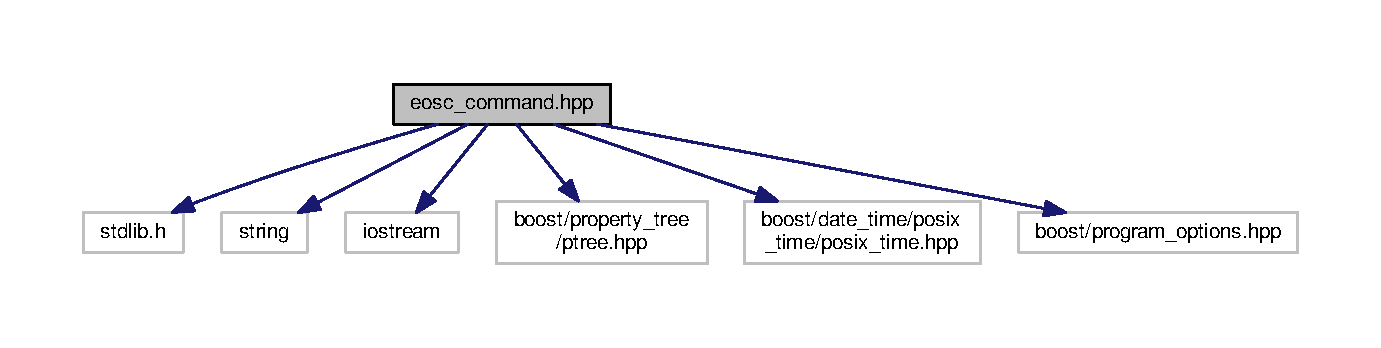
\includegraphics[width=350pt]{eosc__command_8hpp__incl}
\end{center}
\end{figure}
This graph shows which files directly or indirectly include this file\+:\nopagebreak
\begin{figure}[H]
\begin{center}
\leavevmode
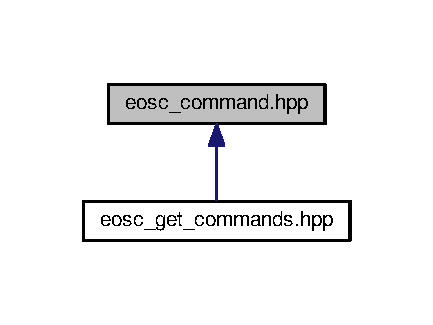
\includegraphics[width=208pt]{eosc__command_8hpp__dep__incl}
\end{center}
\end{figure}
\subsection*{Data Structures}
\begin{DoxyCompactItemize}
\item 
class \hyperlink{classtokenika_1_1eosc_1_1_eosc_command}{tokenika\+::eosc\+::\+Eosc\+Command}
\begin{DoxyCompactList}\small\item\em Basic connection to the blockchain. \end{DoxyCompactList}\item 
class \hyperlink{classtokenika_1_1eosc_1_1_command_options}{tokenika\+::eosc\+::\+Command\+Options}
\begin{DoxyCompactList}\small\item\em Command-\/line wrapper for eosc commands. \end{DoxyCompactList}\end{DoxyCompactItemize}
\subsection*{Macros}
\begin{DoxyCompactItemize}
\item 
\mbox{\Hypertarget{eosc__command_8hpp_a857e89f5c53727699c25d8b17b9c10ed}\label{eosc__command_8hpp_a857e89f5c53727699c25d8b17b9c10ed}} 
\#define {\bfseries E\+O\+S\+C\+\_\+\+E\+R\+R\+OR}~\char`\"{}error\char`\"{}
\item 
\mbox{\Hypertarget{eosc__command_8hpp_ae2080650c6016c93954c88f97fc60e2e}\label{eosc__command_8hpp_ae2080650c6016c93954c88f97fc60e2e}} 
\#define {\bfseries H\+O\+S\+T\+\_\+\+D\+E\+F\+A\+U\+LT}~\char`\"{}localhost\char`\"{}
\item 
\mbox{\Hypertarget{eosc__command_8hpp_aebaae3989ccb20febb9e80449c19f8d3}\label{eosc__command_8hpp_aebaae3989ccb20febb9e80449c19f8d3}} 
\#define {\bfseries P\+O\+R\+T\+\_\+\+D\+E\+F\+A\+U\+LT}~\char`\"{}8888\char`\"{}
\end{DoxyCompactItemize}
\subsection*{Functions}
\begin{DoxyCompactItemize}
\item 
boost\+::posix\+\_\+time\+::ptime {\bfseries tokenika\+::eosc\+::str\+To\+Time} (const std\+::string str)
\begin{DoxyCompactList}\small\item\em Converts E\+OS time string to \textquotesingle{}boost\+::posix\+\_\+time\textquotesingle{}. \end{DoxyCompactList}\item 
void {\bfseries tokenika\+::eosc\+::output} (const char $\ast$label, const char $\ast$format,...)
\begin{DoxyCompactList}\small\item\em Printout formater. \end{DoxyCompactList}\item 
void {\bfseries tokenika\+::eosc\+::call\+Eosd} (std\+::string \hyperlink{classserver}{server}, std\+::string port, std\+::string path, boost\+::property\+\_\+tree\+::ptree \&post\+Json, boost\+::property\+\_\+tree\+::ptree \&json\+Rcv)
\begin{DoxyCompactList}\small\item\em Given a json, eosc\+Command\+Jsongets E\+OS blockchain responce. \end{DoxyCompactList}\item 
{\footnotesize template$<$typename Type $>$ }\\Type {\bfseries tokenika\+::eosc\+::get\+Json\+Path} (boost\+::property\+\_\+tree\+::ptree json, const boost\+::property\+\_\+tree\+::ptree\+::path\+\_\+type \&path)
\begin{DoxyCompactList}\small\item\em Given a json teosc\+Command\+Jsonree, returns the $<$\+Type$>$value of a given path. \end{DoxyCompactList}\item 
boost\+::property\+\_\+tree\+::ptree {\bfseries tokenika\+::eosc\+::string\+To\+Ptree} (std\+::string json)
\begin{DoxyCompactList}\small\item\em Given a text json tree, returns the equivalent {\ttfamily boost ptree}. \end{DoxyCompactList}\end{DoxyCompactItemize}


\subsection{Detailed Description}
Tool for sending transactions and querying state from E\+OS blockchain. 

\begin{DoxyCopyright}{Copyright}
defined in resources/\+L\+I\+C\+E\+N\+S\+E.\+txt Base definitions.
\end{DoxyCopyright}
Defines base classes of the project, and helper methods. 

\subsection{Function Documentation}
\mbox{\Hypertarget{eosc__command_8cpp_file_a522ae193d4a10cba97e59df169dd1da5}\label{eosc__command_8cpp_file_a522ae193d4a10cba97e59df169dd1da5}} 
\index{eosc\+\_\+command.\+hpp@{eosc\+\_\+command.\+hpp}!call\+Eosd@{call\+Eosd}}
\index{call\+Eosd@{call\+Eosd}!eosc\+\_\+command.\+hpp@{eosc\+\_\+command.\+hpp}}
\subsubsection{\texorpdfstring{call\+Eosd()}{callEosd()}}
{\footnotesize\ttfamily void tokenika\+::eosc\+::call\+Eosd (\begin{DoxyParamCaption}\item[{std\+::string}]{server,  }\item[{std\+::string}]{port,  }\item[{std\+::string}]{path,  }\item[{boost\+::property\+\_\+tree\+::ptree \&}]{post\+Json,  }\item[{boost\+::property\+\_\+tree\+::ptree \&}]{json\+Rcv }\end{DoxyParamCaption})}



Given a json, eosc\+Command\+Jsongets E\+OS blockchain responce. 

Given a json tree and a command path (for example {\ttfamily /v1/chain/\+Get\+Info}), and E\+OS blockchain communication port (for example {\ttfamily 8888}), and E\+OS blockchain server name (for example {\ttfamily localhost}), gets E\+OS blockchain responce.


\begin{DoxyParams}{Parameters}
{\em server} & E\+OS blockchain server name \\
\hline
{\em port} & E\+OS blockchain communication port \\
\hline
{\em path} & command path \\
\hline
{\em post\+Json} & json eosc\+Command\+Jsonto be posted \\
\hline
{\em json\+Rcv} & json to be filled with received data \\
\hline
\end{DoxyParams}
\mbox{\Hypertarget{eosc__command_8cpp_file_a2d300c178b2b0dd2e1762fc6c14ee6e1}\label{eosc__command_8cpp_file_a2d300c178b2b0dd2e1762fc6c14ee6e1}} 
\index{eosc\+\_\+command.\+hpp@{eosc\+\_\+command.\+hpp}!get\+Json\+Path@{get\+Json\+Path}}
\index{get\+Json\+Path@{get\+Json\+Path}!eosc\+\_\+command.\+hpp@{eosc\+\_\+command.\+hpp}}
\subsubsection{\texorpdfstring{get\+Json\+Path()}{getJsonPath()}}
{\footnotesize\ttfamily template$<$typename Type $>$ \\
Type tokenika\+::eosc\+::get\+Json\+Path (\begin{DoxyParamCaption}\item[{boost\+::property\+\_\+tree\+::ptree}]{json,  }\item[{const boost\+::property\+\_\+tree\+::ptree\+::path\+\_\+type \&}]{path }\end{DoxyParamCaption})}



Given a json teosc\+Command\+Jsonree, returns the $<$\+Type$>$value of a given path. 


\begin{DoxyTemplParams}{Template Parameters}
{\em Type} & type of the called value \\
\hline
\end{DoxyTemplParams}

\begin{DoxyParams}{Parameters}
{\em json} & json tree \\
\hline
{\em path} & path of the given tree \\
\hline
\end{DoxyParams}
\begin{DoxyReturn}{Returns}
Type 
\end{DoxyReturn}
\mbox{\Hypertarget{eosc__command_8cpp_file_a03be7086d7980dc8c27b7aaaf8973771}\label{eosc__command_8cpp_file_a03be7086d7980dc8c27b7aaaf8973771}} 
\index{eosc\+\_\+command.\+hpp@{eosc\+\_\+command.\+hpp}!output@{output}}
\index{output@{output}!eosc\+\_\+command.\+hpp@{eosc\+\_\+command.\+hpp}}
\subsubsection{\texorpdfstring{output()}{output()}}
{\footnotesize\ttfamily void tokenika\+::eosc\+::output (\begin{DoxyParamCaption}\item[{const char $\ast$}]{label,  }\item[{const char $\ast$}]{format,  }\item[{}]{... }\end{DoxyParamCaption})}



Printout formater. 

For example, {\ttfamily output(\char`\"{}timestamp\char`\"{}, \char`\"{}\%s\char`\"{}, \char`\"{}2017-\/07-\/18\+T20\+:16\+:36\char`\"{})} produces {\ttfamily \#\# timestamp\+: 2017-\/07-\/18\+T20\+:16\+:36}


\begin{DoxyParams}{Parameters}
{\em label} & \\
\hline
{\em format} & \\
\hline
{\em ...} & \\
\hline
\end{DoxyParams}
\mbox{\Hypertarget{eosc__command_8cpp_file_a0ce29794654e913a1069e28530f4fe46}\label{eosc__command_8cpp_file_a0ce29794654e913a1069e28530f4fe46}} 
\index{eosc\+\_\+command.\+hpp@{eosc\+\_\+command.\+hpp}!string\+To\+Ptree@{string\+To\+Ptree}}
\index{string\+To\+Ptree@{string\+To\+Ptree}!eosc\+\_\+command.\+hpp@{eosc\+\_\+command.\+hpp}}
\subsubsection{\texorpdfstring{string\+To\+Ptree()}{stringToPtree()}}
{\footnotesize\ttfamily boost\+::property\+\_\+tree\+::ptree tokenika\+::eosc\+::string\+To\+Ptree (\begin{DoxyParamCaption}\item[{std\+::string}]{json }\end{DoxyParamCaption})}



Given a text json tree, returns the equivalent {\ttfamily boost ptree}. 


\begin{DoxyParams}{Parameters}
{\em json} & \\
\hline
\end{DoxyParams}
\begin{DoxyReturn}{Returns}
boost\+::property\+\_\+tree\+::ptree 
\end{DoxyReturn}
\mbox{\Hypertarget{eosc__command_8cpp_file_af36b60963055656769794bd43927654c}\label{eosc__command_8cpp_file_af36b60963055656769794bd43927654c}} 
\index{eosc\+\_\+command.\+hpp@{eosc\+\_\+command.\+hpp}!str\+To\+Time@{str\+To\+Time}}
\index{str\+To\+Time@{str\+To\+Time}!eosc\+\_\+command.\+hpp@{eosc\+\_\+command.\+hpp}}
\subsubsection{\texorpdfstring{str\+To\+Time()}{strToTime()}}
{\footnotesize\ttfamily boost\+::posix\+\_\+time\+::ptime tokenika\+::eosc\+::str\+To\+Time (\begin{DoxyParamCaption}\item[{const std\+::string}]{str }\end{DoxyParamCaption})}



Converts E\+OS time string to \textquotesingle{}boost\+::posix\+\_\+time\textquotesingle{}. 

E\+OS time is a string, for example {\ttfamily 2017-\/07-\/18\+T20\+:16\+:36}. For processing, it is converted to the boost {\ttfamily ptime}.


\begin{DoxyParams}{Parameters}
{\em str} & E\+OS time string. \\
\hline
\end{DoxyParams}
\begin{DoxyReturn}{Returns}
boost\+::posix\+\_\+time\+::ptime 
\end{DoxyReturn}

\hypertarget{eosc__get__commands_8hpp}{}\section{eosc\+\_\+get\+\_\+commands.\+hpp File Reference}
\label{eosc__get__commands_8hpp}\index{eosc\+\_\+get\+\_\+commands.\+hpp@{eosc\+\_\+get\+\_\+commands.\+hpp}}
{\ttfamily \#include $<$boost/date\+\_\+time/posix\+\_\+time/posix\+\_\+time.\+hpp$>$}\newline
{\ttfamily \#include $<$boost/property\+\_\+tree/ptree.\+hpp$>$}\newline
{\ttfamily \#include \char`\"{}../eosc\+\_\+config.\+h\char`\"{}}\newline
{\ttfamily \#include \char`\"{}eosc\+\_\+command.\+hpp\char`\"{}}\newline
Include dependency graph for eosc\+\_\+get\+\_\+commands.\+hpp\+:
\nopagebreak
\begin{figure}[H]
\begin{center}
\leavevmode
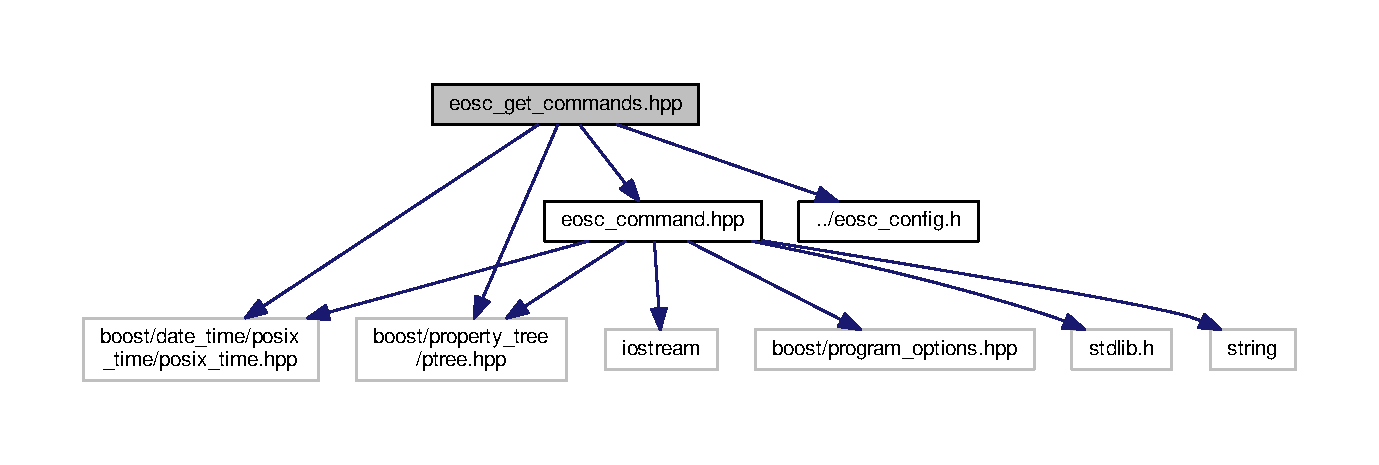
\includegraphics[width=350pt]{eosc__get__commands_8hpp__incl}
\end{center}
\end{figure}
\subsection*{Data Structures}
\begin{DoxyCompactItemize}
\item 
class \hyperlink{classtokenika_1_1eosc_1_1_get_info}{tokenika\+::eosc\+::\+Get\+Info}
\begin{DoxyCompactList}\small\item\em Get current blockchain information. \end{DoxyCompactList}\item 
class \hyperlink{classtokenika_1_1eosc_1_1_get_info_options}{tokenika\+::eosc\+::\+Get\+Info\+Options}
\item 
class \hyperlink{classtokenika_1_1eosc_1_1_get_block}{tokenika\+::eosc\+::\+Get\+Block}
\begin{DoxyCompactList}\small\item\em Retrieve a full block from a blockchain. \end{DoxyCompactList}\item 
class \hyperlink{classtokenika_1_1eosc_1_1_get_block_options}{tokenika\+::eosc\+::\+Get\+Block\+Options}
\end{DoxyCompactItemize}


\subsection{Detailed Description}
Definitions for get-\/type commands.

Defines command line options. 
%--- End generated contents ---

% Index
\backmatter
\newpage
\phantomsection
\clearemptydoublepage
\addcontentsline{toc}{chapter}{Index}
\printindex

\end{document}
